\documentclass[12pt,a4paper]{article}

% ─── Packages ────────────────────────────────────────────────────
\usepackage[utf8]{inputenc}
\usepackage[T1]{fontenc}
\usepackage{lmodern}
\usepackage[margin=1in]{geometry}
\usepackage{graphicx}
\usepackage[titles]{tocloft}
\usepackage{hyperref}
\usepackage{booktabs}
% tabularx removed — using tabular with p{} columns
\usepackage{enumitem}
\usepackage{xcolor}
\usepackage{titlesec}
\usepackage{parskip}
\usepackage{fancyhdr}
\usepackage{microtype}
\usepackage{cite}
\usepackage{listings}

\usepackage{tikz}
\usetikzlibrary{shapes.geometric, arrows.meta, positioning, shadows.blur}


% ─── Code listing style ───────────────────────────────────────────
\lstdefinelanguage{EEPJson}{
  morestring=[b]",
  morecomment=[l]{//},
  morekeywords={true,false,null},
  sensitive=false,
}
\lstdefinelanguage{EEPHttp}{
  morecomment=[l]{//},
  morekeywords={GET,POST,PUT,DELETE,HTTP,EEP-Version,EEP-Agent-DID,EEP-Signature,EEP-Nonce,Content-Type,Authorization,Link,Retry-After},
  morestring=[b]",
}
\lstdefinestyle{eepcode}{
  backgroundcolor=\color{gray!8},
  basicstyle=\small\ttfamily,
  breaklines=true,
  breakatwhitespace=false,
  frame=single,
  framesep=5pt,
  rulecolor=\color{gray!50},
  numbers=none,
  keywordstyle=\color{blue!70!black}\bfseries,
  stringstyle=\color{orange!80!black},
  commentstyle=\color{green!50!black}\itshape,
  showstringspaces=false,
  tabsize=2,
  captionpos=b,
  xleftmargin=4pt,
  xrightmargin=4pt,
}
\lstset{style=eepcode}


% ─── Hyperref setup ──────────────────────────────────────────────
\hypersetup{
    colorlinks=true,
    linkcolor=blue!60!black,
    citecolor=blue!60!black,
    urlcolor=blue!60!black,
    pdftitle={The Entity Engagement Protocol (EEP) Whitepaper},
    pdfauthor={Dr. Ugur Cekmez},
}
% Table of contents: avoid section titles and page numbers crowding (reviewer feedback)
\cftsetpnumwidth{2.85em}
\setlength{\cftsecnumwidth}{3.0em}
\setlength{\cftsubsecnumwidth}{3.8em}
\setlength{\cftsubsubsecnumwidth}{4.4em}
\makeatletter
\renewcommand{\@pnumwidth}{2.85em}
\renewcommand{\@tocrmarg}{4.5em plus 1fil}
\renewcommand{\l@subsection}{\@dottedtocline{2}{3.6em}{4.0em}}
\renewcommand{\l@subsubsection}{\@dottedtocline{3}{7.6em}{4.6em}}
\makeatother

% ─── Section styling ─────────────────────────────────────────────
\titleformat{\section}{\Large\bfseries}{\thesection}{1em}{}
\titleformat{\subsection}{\large\bfseries}{\thesubsection}{1em}{}
\titleformat{\subsubsection}{\normalsize\bfseries}{\thesubsubsection}{1em}{}

% ─── Header/Footer ───────────────────────────────────────────────
\pagestyle{fancy}
\fancyhf{}
\fancyhead[L]{\small\textit{The Entity Engagement Protocol (EEP)}}
\fancyhead[R]{\small\textit{Whitepaper v0.1}}
\fancyfoot[C]{\thepage}
\renewcommand{\headrulewidth}{0.4pt}

% L column type removed with tabularx

\begin{document}

% ─── Title Page ──────────────────────────────────────────────────
\begin{titlepage}
\centering
\vspace*{2cm}

{\Huge\bfseries The Entity Engagement Protocol (EEP)\par}
\vspace{1cm}
{\Large\itshape Architecting the Identity, State and Commerce Layer\\for the Global Agentic Web\par}
\vspace{4cm}

{\Large Dr. Ugur Cekmez\par}
{\small Professor, Munich University of Digital Technologies and Applied Sciences\par}
\vspace{0.5em}
\vspace{2.0cm}
{\large https://eep.dev\par}
\vspace{2.0cm}
{\large May 2026\par}

\vfill
{\small Version 0.1}
\end{titlepage}

% ─── Table of Contents ───────────────────────────────────────────
\tableofcontents
\newpage

% ─── Abstract ───────────────────────────────────────────────────
\section*{Abstract}
\addcontentsline{toc}{section}{Abstract}

The internet was built for human eyes. Visual layouts, interactive buttons, unstructured text. Thirty years of design choices that made complete sense when the reader was a person. But Large Language Models have stopped being chatbots; they are turning into agents that plan, decide and execute, and our human-centric infrastructure is breaking under them. Today an agent that wants a single price point has to scrape and guess its way through thousands of lines of HTML. It is slow, it breaks all the time, and it burns absurd amounts of compute and tokens.

The Entity Engagement Protocol (EEP) goes further than fixing the data format. It is the infrastructure layer for an \textbf{Agent Ecosystem}: a network of agents, entities and data providers that interact continuously to exchange value. Access here is rarely binary, public or private. It is governed by programmable, machine-verifiable requirements: payment, trust credentials, signed agreements, data exchange. EEP collapses those patterns into one network-layer specification, so agents and publishers can rely on a single machine-readable contract.

Under the hood, the protocol uses a three-layer stack. Layer 1 carries static state (structured data like JSON, Markdown, TOON). Layer 2 carries real-time streaming (Server-Sent Events and Webhooks). Layer 3 carries bidirectional negotiation (WebSockets for commerce). The whole thing sits on Decentralized Identifiers (DIDs) \cite{ref5} and W3C Verifiable Credentials 2.0 \cite{ref10}, which give machine-to-machine interaction the trust and sovereignty it actually requires. Alongside the normative specification, the open-source project ships a dual-runtime reference deployment, the \texttt{eep-setup} artifact generator, Node and Python middleware, machine-readable setup and compliance reports, and operator documentation for fast proofs and CI verification. The reference implementation, the middleware libraries and the \texttt{@eep-dev/setup-cli} package (\texttt{eep-setup}) are released under the \textbf{Apache License, version 2.0}, matching the normative specification repository. This paper explains why the infrastructure is needed now, how it works, and what it makes possible. Most of what privacy and AI-governance regulators ask for maps onto concrete protocol artifacts: declared purposes, retention limits, delegation proofs, signed commerce events. That is what compliance-oriented design at the wire level means here, as opposed to narrative assurances after the fact.

\textbf{Federated trust.} Registry federation (Section~4.5) lets other registry operators, not only \texttt{eep.dev}, issue trust and conformance credentials that agents verify via the issuer chain. The bootstrapping registry helps discovery; it is not a single control point for whether two parties can interact when they already have manifests, DIDs and trust anchors out of band.


\noindent\textit{How to read this document.} If you are a developer building EEP endpoints, focus on the Protocol Architecture, Session Persistence, Security and Conformance Testing sections. If you are a platform operator adopting the shipped reference stack or the \texttt{@eep-dev/setup-cli} tool (\texttt{eep-setup}), the Reference Implementation, Setup Tooling and Verification section is the main one, together with the deployment and five-minute proof guides in the repository. Strategists and investors will find the motivation in Sections 1--2, use cases in Section~11, and the self-regulating standard argument in Section~15. Enterprise architects evaluating adoption should start with the Interoperability and Regulatory Compliance sections. Researchers interested in the agent economy will want the Agent Economy, Privacy by Design and Price Discovery sections.


% ═══════════════════════════════════════════════════════════════════
\part*{Part~I:~The~Problem}
\addcontentsline{toc}{part}{Part I: The Problem}
\section{The Unavoidable Agentic Shift \& Resource Scarcity}

The shift toward an Agentic Web is not speculative. It is happening in production. Market projections put autonomous AI at USD 139 billion by 2034, on the back of enterprises that already have agents running procurement, negotiating contracts and managing supply chains, not just drafting emails \cite{ref1, ref7, ref8}.

There is a serious problem with all of this: the work we expect these agents to do is at odds with the infrastructure we are forcing them to use.

\subsection{The ``HTML Tax'' and Compute Scarcity}

When Nvidia CEO Jensen Huang tied corporate revenue directly to raw compute generation in early 2026, he was not exaggerating: ``compute equals revenues'' \cite{ref2}. The basic unit of that compute is the generated token.

Tokens are finite, expensive and energetically heavy. When an agent hits a standard corporate website today, it has to ingest thousands of lines of HTML, CSS classes and JavaScript tags just to find a single price point. We call this the \textit{HTML Tax}. Reading raw HTML inflates token consumption by roughly 80\% compared with formats like Markdown \cite{ref3}. Published Token-Oriented Object Notation (TOON) benchmarks report token savings on the order of 40\% versus JSON in comparable agent-tool scenarios \cite{ref31}. The International Energy Agency estimates that a single generative AI query already consumes about ten times the electricity of a traditional Google search \cite{ref4}.

The waste is not only financial. Extra tokens and extra round-trips mean extra generation, extra cooling and extra network work for the same factual outcome, which is why \textit{green IT} and carbon-aware operations teams have the same incentive as CFOs: fewer joules per correct answer. EEP does not replace sustainability programs. It attacks the same root cause as cost discipline: stop paying the \textit{HTML Tax} when structured state and push signals already exist.

Scaling this scraping paradigm to billions of daily agent transactions is not just difficult; it is impossible. We are walking straight into compute scarcity. Switching protocols is not a nice-to-have developer feature; it is an economic requirement. Agents need clean, dense, structured data because they cannot afford to waste context windows on visual layouts that were designed for humans.

Separately from cost, \emph{generative engine optimization} (GEO) research looks at how sources are selected and cited inside LLM-mediated answers; benchmarked evaluations report large visibility swings when content is structured for retrieval rather than presentation \cite{ref33}. Native content negotiation toward dense Layer~1 formats (Section~\ref{sec:philosophy}) pushes in the same direction: more factual signal per token, less layout noise.

% ═══════════════════════════════════════════════════════════════════
\section{The Agent Ecosystem: Why Agents Must Interact}

Today, AI assistants are mostly tools that developers use. That is changing fast. Within a few years, individuals, businesses and institutions will run agents for a long list of purposes. Some will be generic, like a personal scheduling agent. Some will be very specialized, like a pharmaceutical regulatory compliance agent. Most of them, whatever their purpose, will hit a wall where they cannot do their work alone.

A personal finance agent needs pricing data from banks. A compliance agent needs regulatory updates from government entities. A research agent needs access to paywalled datasets. A creative agent needs licensing information before it can republish content. In each case the agent has to interact with an external party, and the interaction has to happen autonomously, reliably and on legally defensible terms.

This is the real problem EEP addresses. The point is not efficient data formats, although it does deliver those. The point is the conditions under which agents can actually function in the world: acquiring what they need, proving who they are, agreeing to terms they must accept, and exchanging what they are asked for.

\subsection{The Access Spectrum}

Not all data is free and not all gating is about money. EEP models data access as a spectrum:

\begin{itemize}
    \item \textbf{Public:} Available to any agent, no credentials required.
    \item \textbf{Trust-gated:} Restricted to agents that can present a verifiable proof of trustworthiness or affiliation (e.g., ``only verified research agents may access this dataset'').
    \item \textbf{Agreement-gated:} Requires the requesting agent to cryptographically sign a specific license or terms of service before access is granted (e.g., ``educational use only, no commercial redistribution'').
    \item \textbf{Data-exchange-gated:} Requires the requesting agent to provide specific data about itself or its owner in exchange for the requested payload (e.g., ``provide your usage intent and organization type'').
    \item \textbf{Payment-gated:} Requires a verifiable proof of micropayment, typically via a smart contract transaction.
    \item \textbf{Combined:} Any combination of the above (e.g., a credential \textit{and} a signed agreement \textit{and} a payment).
\end{itemize}

EEP covers all of these in one protocol layer. Entities configure their access gates declaratively. Agents parse and satisfy the requirements autonomously. Humans do not need to be in the loop unless the entity explicitly demands it.

% ═══════════════════════════════════════════════════════════════════
\part*{Part~II:~The~Protocol}
\addcontentsline{toc}{part}{Part II: The Protocol}
\section{The EEP Core Philosophy: DIDs and Event-Driven State}
\label{sec:philosophy}

EEP assumes the ``web page'' is dead. The internet is a network of \textbf{Entities} (people, organizations, AI agents, products, knowledge bases) that emit structured \textbf{Events}.

The protocol rests on three ideas:

\begin{enumerate}
    \item \textbf{Identity is decentralized.} Every entity in an EEP network is a sovereign participant identified by a W3C Decentralized Identifier (DID) \cite{ref5}. Agents do not log in with usernames and passwords. They authenticate cryptographically.
    \item \textbf{Data is format-agnostic.} EEP relies on HTTP content negotiation (\texttt{Accept} headers). Agents ask for what they need. A reasoning agent might request \texttt{text/markdown} because LLMs read its structural cues well. A low-latency parser might request \texttt{text/toon} (Token-Oriented Object Notation) to squeeze the most data into a tight context window.
    \item \textbf{Interaction is event-driven.} Polling REST APIs wastes resources. In an agent economy, state has to be pushed. EEP requires publishers to emit CloudEvents-formatted \cite{ref6} payloads when state changes, so the network shifts from pull-based scraping to push-based synchronization.
\end{enumerate}

\noindent\textbf{Decentralized by design.}
W3C DIDs and federated registries (Section~4.5) are not cosmetic. They let operators publish manifests and trust anchors under their own domains, and they let agents verify issuer chains, so no single vendor becomes the unavoidable gate for ``the'' agent internet. Discovery can boot through \texttt{eep.dev} or through another federated registry the relying party already trusts. The protocol aims at portable participation, not a walled garden with extra APIs.

\paragraph{Wire format vs.\ shared meaning.}
EEP is flexible on \emph{representation} at Layer~1 (content negotiation for JSON, Markdown, TOON and similar). The flexibility does not remove the need for \emph{semantic alignment} in commerce and entitlement objects. Bilateral \texttt{offer}/\texttt{counter} flows, invoices and \texttt{data\_request} responses SHOULD carry JSON-LD \texttt{@context} (and, where helpful, reuse stable public vocabularies such as Schema.org) or other manifest-declared schema identifiers, so that both sides refer to the same currency, unit, SKU, quota and retention semantics. W3C Verifiable Credentials already anchor meaning via \texttt{@context}; commerce and pricing profiles SHOULD follow the same pattern when publishers register machine-readable profiles in their manifests.

% ═══════════════════════════════════════════════════════════════════
\section{Discovery and the EEP Registry}

For an Agent Ecosystem to function, agents have to find the EEP endpoints of entities they have never spoken to before. Static configuration does not scale. EEP defines a two-tier discovery model: a DNS-based well-known path for entity-side self-declaration, and \texttt{eep.dev} as the protocol's official bootstrapping registry.

\subsection{Well-Known Self-Declaration}

Any entity that speaks EEP must expose a machine-readable manifest at a standardized path:

\begin{lstlisting}[language=EEPJson,style=eepcode]
https://{domain}/.well-known/eep.json
\end{lstlisting}

The manifest declares the entity's DID, its supported EEP version, the URLs for each protocol layer (Layer 1 state endpoint, Layer 2 subscribe endpoint, Layer 3 WebSocket endpoint), its supported content types and its gate tiers. The path follows RFC~8615 \cite{ref20}, so any agent that knows the domain can find it immediately.

This is decentralized on purpose: no central registry is required for an agent to interact with an entity whose domain it already knows. The manifest is the single source of truth. It can be served statically and cached aggressively.

\subsection{Manifests, sitemaps and generative retrieval}

Traditional SEO used HTML links and XML \texttt{sitemap.xml} files so crawler-based search engines could enumerate pages. Conversational and retrieval-augmented systems pose a different problem: how do automated fetchers get \emph{dense, current, permissioned} facts without re-parsing entire sites for every answer? Work on \emph{generative engine optimization} (GEO) frames this as making sources easier to retrieve and cite inside LLM outputs \cite{ref33}. The EEP manifest is not a ranking gimmick. It is a deterministic declaration of DIDs, protocol layers, gates and content types. That cuts guesswork for autonomous clients and for pipelines that hydrate generative answers, alongside (not instead of) classic discovery documents.

\subsection{Dynamic Capability Discovery}

Early agent frameworks like the Model Context Protocol (MCP) hit a clear wall when transmitting large, static tool registries: context-window exhaustion. EEP works around this with \textbf{Dynamic Capability Discovery}. Implementations with large catalogs can expose paginated or queryable capability surfaces so agents pull only what they need for the current task, rather than downloading a monolithic manifest. The base \nolinkurl{/.well-known/eep.json} file remains the root discovery document. Extended discovery is an optional overlay that publishers can choose to offer.


\subsection{eep.dev: The Protocol Registry and Bootstrapping Hub}

For agents discovering entities they have never seen before, EEP runs \texttt{eep.dev} as the protocol's official registry. Eep.dev does four things:

\begin{enumerate}
    \item \textbf{Entity Registry.} Organizations and individuals register their EEP-compliant endpoints at \texttt{eep.dev/registry}. Registrations are verified by confirming the presence of a valid \texttt{/.well-known/eep.json} manifest. Agents query the registry using a standard REST API, with full-text search, category filters, gate type filters and trust score thresholds.

    \item \textbf{Capability Discovery API.} An agent building a procurement workflow can query \texttt{eep.dev/discover?category=supply-chain\&gate=payment\&supports=sse} for a filtered list of entities that match its exact requirements. The API returns the entity's DID, manifest URL and a summary of its declared capabilities.

    \item \textbf{Trust Anchor.} Eep.dev issues Verifiable Credentials to registered entities that pass integrity checks (e.g., DID ownership proof, manifest consistency). The credentials act as a baseline trust signal that agents can rely on when making first-contact decisions.

    \item \textbf{Protocol Namespace.} All EEP event type strings (e.g., \texttt{com.example.entity.updated}) are declared and documented in the eep.dev namespace registry. This prevents naming collisions and gives agents one authoritative reference for interpreting unfamiliar event types.
\end{enumerate}

Trust Anchor credentials are not exclusive to the \texttt{eep.dev} operator. Under the Registry Federation model (Section~4.5), other registries that hold a valid Registry Federation Credential may issue their own trust and conformance credentials; agents verify the issuer chain, not a single hostname.

One more thing: \texttt{eep.dev} is not a mandatory dependency. The well-known manifest means any two parties can interact with zero involvement from eep.dev. The registry accelerates discovery; it is not a chokepoint for the protocol. If eep.dev went offline tomorrow, no existing agent-entity interaction would break.

\textbf{Operational note.} Before citing \texttt{eep.dev/...} URLs in public materials, operators should make sure the domain resolves to maintained infrastructure (or transparent redirects) so readers do not hit dead links. A minimal landing page or redirect is enough while broader services roll out.

\subsection{DNS and Link Header Discovery}

For environments where the \texttt{/.well-known/} path is not accessible (e.g., non-web entities like IoT devices), EEP also supports discovery through HTTP \texttt{Link} headers with \texttt{rel=``eep''} or through DNS TXT records of the form:

\begin{lstlisting}[language=EEPJson,style=eepcode]
_eep.example.com. 300 IN TXT "v=eep1; manifest=https://api.example.com/.well-known/eep.json"
\end{lstlisting}

This allows any EEP entity, regardless of how its infrastructure is structured, to be discoverable by a compliant agent.

\subsection{Registry Federation}

As EEP adoption grows, \texttt{eep.dev} cannot remain the only authorized registry, and it should not be. Jurisdictions, industry verticals and large-scale operators will want to run their own. A European financial services consortium might run \texttt{eep.eu}. A healthcare industry body might run \texttt{eep-health.org}. Each would apply sector-specific trust criteria that a general-purpose registry has no business enforcing.

EEP defines a \textbf{Registry Federation Protocol} for this case. Any registry that wants to federate with the EEP ecosystem must:

\begin{enumerate}
    \item Publish its own registry manifest at \texttt{/.well-known/eep-registry.json}, declaring its DID, its trust criteria, its conformance tier requirements and the scope of entities it registers (by geography, sector or capability).
    \item Register itself at \texttt{eep.dev/registries}, where the EEP Standards Committee issues it a \textbf{Registry Federation Credential}: a Verifiable Credential confirming it operates according to the EEP Registry Federation Protocol.
    \item Implement a cross-registry resolution API: when an agent queries a federated registry for an entity not in its own index, the registry must attempt to resolve via peered registries before returning a not-found response.
\end{enumerate}

Agents that interact with entities on a federated registry verify the registry's Federation Credential before trusting its Trust Anchor VCs. The result is a \textbf{web of trust} across registry operators, decentralized and not dependent on eep.dev staying online, with a common cryptographic standard for what ``trusted'' means.

Conformance Credentials issued by federated registries are cross-verifiable: a Conformance VC issued by \texttt{eep.eu} with a valid Federation Credential is implicitly accepted by any agent that trusts the EEP federation root. No manual allowlisting required.

\textbf{Registry operator economics.} We do not assume federation infrastructure runs on goodwill alone. Federated registries SHOULD publish machine-readable \texttt{economics} metadata in \texttt{/.well-known/eep-registry.json}: registration fees, capability-query quotas with paid tiers, optional micro-staking or proof-of-payment/proof-of-work challenge policies. Agents use this signal to assess sustainability and Sybil resistance. Absence is a trust downgrade, not a hard failure.

% ═══════════════════════════════════════════════════════════════════

\begin{figure}[htbp]
\centering
\resizebox{\textwidth}{!}{
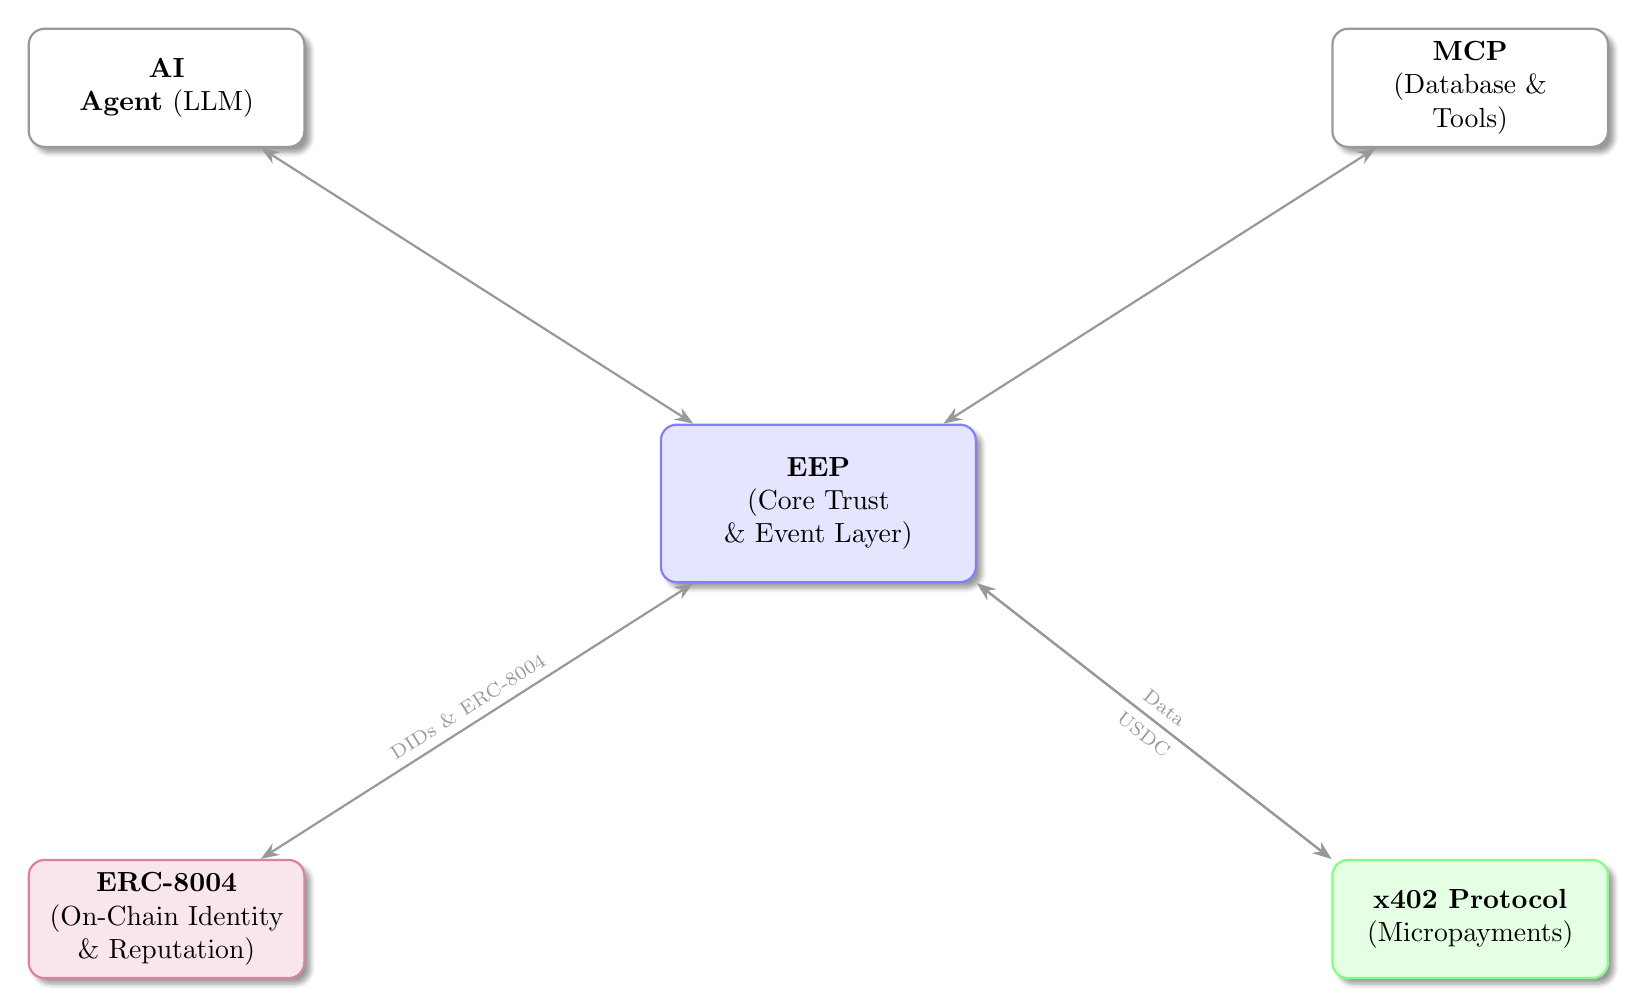
\begin{tikzpicture}[
    node distance=3.5cm and 4.5cm,
    box/.style={rectangle, draw=black!40, fill=white, thick, rounded corners=2mm, 
                minimum width=3.5cm, minimum height=1.5cm, align=center, blur shadow={shadow blur steps=5}},
    centerbox/.style={box, fill=blue!10, draw=blue!50, minimum width=4cm, minimum height=2cm},
    arrow/.style={-{Stealth[scale=1.2]}, thick, color=gray!80, dashed},
    doublearrow/.style={<->, >=Stealth, thick, color=gray!80}
]

% Nodes
\node[centerbox] (eep) {\textbf{EEP} \\ (Core Trust \\\& Event Layer)};

\node[box] (llm) [above left=of eep] {\textbf{AI} \\ \textbf{Agent} (LLM)};
\node[box] (mcp) [above right=of eep] {\textbf{MCP} \\ (Database \& \\ Tools)};

\node[box, fill=purple!10, draw=purple!50] (erc) [below left=of eep] {\textbf{ERC-8004} \\ (On-Chain Identity \\\& Reputation)};
\node[box, fill=green!10, draw=green!50] (x402) [below right=of eep] {\textbf{x402 Protocol} \\ (Micropayments)};

% Arrows
\draw[doublearrow] (llm) -- (eep);
\draw[doublearrow] (mcp) -- (eep);
\draw[doublearrow] (eep) -- node[above, sloped, font=\scriptsize] {DIDs \& ERC-8004} (erc);
\draw[doublearrow] (eep.south east) -- node[above, sloped, font=\scriptsize] {Data} (x402.north west);
\draw[doublearrow] (x402.north west) -- node[below, sloped, font=\scriptsize] {USDC} (eep.south east);

\end{tikzpicture}
}
\caption{Reference integration diagram: EEP as the M2M trust and event layer between LLM agents, MCP tool hosts, on-chain identity (ERC-8004 \cite{ref28}) and micropayment settlement (x402 \cite{ref27}), with DIDs \cite{ref5} as the shared identity anchor.}
\label{fig:architecture}
\end{figure}

\section{Protocol Architecture: The Triple Protocol Stack}

Most current APIs offer one mode of interaction, normally synchronous REST. EEP assumes agents need both historical context (static data) and immediate awareness (real-time data). So EEP requires a ``Triple Protocol'' implementation.

\subsection{Layer 1: State Resolution (REST)}
State resolution lets agents read the current state of an entity on demand. When an agent hits an entity's endpoint (e.g., \texttt{GET /:type/:username}), the publisher returns the entity's baseline profile, capabilities and discovery links (notably the \texttt{rel=``subscribe''} link). This layer is for initial ingestion only.

\subsection{Layer 2: Signal Stream (SSE and Webhooks)}
The Signal Stream is unidirectional and real-time. This is how agents watch the world.
\begin{itemize}
    \item \textbf{SSE (Server-Sent Events).} For a lightweight, continuous connection, EEP mandates an SSE endpoint \cite{ref21}. Agents subscribe to specific entity events (e.g., \texttt{events=com.example.entity.updated,com.example.trust.*}). Publishers MUST support the \texttt{Last-Event-ID} header, typically backed by Redis Streams or similar, to replay any missed events when an agent drops its connection.
    \item \textbf{Webhooks.} For asynchronous agents or serverless workflows, EEP supports webhook delivery with WebSub intent verification to prevent abuse, HMAC-SHA256 signatures on the payload, and exponential backoff retry policies.
\end{itemize}

\subsection{Layer 3: Network Pulse (WebSockets)}
Layer 2 is read-only. Layer 3 handles bidirectional, interactive scenarios: Agent-to-Agent (A2A) task negotiation, continuous chat, autonomous commerce. All messages are structured JSON envelopes that contain a \texttt{type}, an \texttt{action} and a monotonically increasing \texttt{seq} number. With these in place, agents can orchestrate multi-turn interactions, detect network gaps and request replays as needed.

\subsubsection{Reconnection, gaps and state growth}
Layer~3 is not an unbounded server-side buffer for client state. Publishers SHOULD cap per-connection history and rely on the same back-pressure principle as Layer~2: if a client falls too far behind, the server closes the WebSocket with application code \texttt{4000} (slow consumer) rather than holding on to an ever-growing queue. This mirrors the Layer~2 policy of terminating overloaded streams instead of letting memory grow without bound.

For ordering and catch-up, Layer~3 uses per-channel monotonic \texttt{seq} values (not the SSE \texttt{Last-Event-ID} header). When a client observes a gap in \texttt{seq}, it issues a \texttt{system}/\texttt{replay} envelope asking for messages from a prior sequence number; the normative rules are in the specification (\S6.3). Long-lived sessions use JWT re-authentication (\S6.4) so that a reconnect after transport failure re-establishes trust before replay resumes. Between them, \texttt{seq}+replay+session refresh give a practical reconciliation story without pretending that WebSockets are a durable infinite log.

\paragraph{Replay buffer bounds.}
Slow-consumer handling (close code \texttt{4000}) prevents unbounded queues, but replay needs a cap too. Publishers SHOULD declare per-channel replay limits in the Layer~1 manifest (e.g., maximum retained messages or maximum age); normative field names and error behavior are defined in the companion specification (Layer~3, replay retention). Implementations MUST NOT retain unbounded backlogs. If a client asks for history older than the retained window, the server SHOULD return an explicit error so the client snapshots or reconciles from Layer~1 state instead of assuming an infinite server-side log.

\begin{table}[h!]
\centering
\caption{Qualitative traffic profile: Layer~1 vs Layer~3 (typical agent workloads)}
\label{tab:layer-cost}
\renewcommand{\arraystretch}{1.25}
\begin{tabular}{|p{3.0cm}|p{5.5cm}|p{5.5cm}|}
\hline
\textbf{Aspect} & \textbf{Layer 1 (state / REST)} & \textbf{Layer 3 (WebSocket pulse)} \\
\hline
Interaction shape & Request/response; short JSON documents & Persistent channel; bidirectional envelopes \\
\hline
Server memory & Scoped to request handling & Bounded channels; replay + back-pressure instead of unbounded buffers \\
\hline
Token / compute angle & Favours compact representations (TOON, Markdown) for each response & Higher steady-state overhead (session, heartbeats, commerce state); pays for negotiation and multi-turn semantics \\
\hline
\end{tabular}
\end{table}

\subsection{Version Negotiation}

As EEP evolves, agents and publishers will end up running different versions of it. EEP handles this autonomously through a lightweight content-negotiation approach.

Every EEP entity declares the protocol versions it supports in its \texttt{/.well-known/eep.json} manifest:

\begin{lstlisting}[language=EEPJson,style=eepcode]
{
  "eep_versions": ["0.1", "0.2"],
  "preferred_version": "0.2"
}
\end{lstlisting}

When an agent initiates a request, it includes an \texttt{EEP-Version} header listing the versions it supports, in preference order. The publisher replies with an \texttt{EEP-Version} header confirming the chosen version (the highest mutually supported one). If no overlap exists, the publisher responds with \texttt{HTTP 505} and the full list of its supported versions, so the agent can update or fall back.

EEP recognises two classes of change:
\begin{itemize}
    \item \textbf{Non-breaking.} New optional fields, new event types, new gate requirement types. Older agents safely ignore unknown fields. No version bump required in the minor range.
    \item \textbf{Breaking.} Changes to the gate challenge format, session token structure or signature algorithm requirements. These will bump the major version once EEP reaches 1.x. Until then, breaking changes are reflected in draft increments; a publisher that supports multiple draft lines runs both stacks in parallel during the deprecation window (minimum 12 months). Ecosystem-facing notice of a breaking change in the \texttt{0.x} line follows \texttt{GOVERNANCE.md} (advance notice before consumers are expected to migrate). The 12-month figure is a minimum overlap for operators running dual implementations; it is not a substitute for that notice cadence.
\end{itemize}

Negotiation happens autonomously on every first-contact request. No human configuration is required.

% ═══════════════════════════════════════════════════════════════════
\section{Agent Session Persistence}

Not every agent-entity interaction is a single request. A personal finance agent might hold a months-long subscription to a bank's rate feed. A legal agent managing an ongoing contract might come back to the same entity dozens of times over weeks. A logistics agent tracking a shipment carries context across hundreds of event updates.

These are relationships, not transactions. EEP defines a \textbf{Session Persistence} model that standardizes how long-lived agent-entity relationships are established, maintained and torn down.

\subsection{Session Tokens and Relationship Context}

Once an agent completes a gate requirement (credential, agreement, data exchange or payment), the publisher issues a signed \textbf{Session Token}: a short-lived JWT-like structure signed by the publisher's DID private key. The session token carries:

\begin{itemize}
    \item The agent's DID. The session is bound to this identity.
    \item The tier or tiers the agent has access to.
    \item An expiry time (\texttt{exp}). Expiry can be anything from a few minutes to several months, depending on the relationship.
    \item A \texttt{refresh\_threshold} after which the agent should proactively request renewal.
    \item A \texttt{context\_id} the agent uses to resume any interrupted operation (e.g., replaying missed events from a specific position).
\end{itemize}

The agent stores this token (encrypted, in its own secure store) and presents it on later requests via the \texttt{Authorization: EEP-Session} header. The publisher validates the token signature against the issuing DID key before serving the request. The full gate verification flow is not repeated.

\subsection{Relationship Renewal and Agreement Revocation}

When a session token nears its \texttt{refresh\_threshold}, the agent requests renewal proactively. If the underlying gate requirements have not changed, renewal is automatic and only the current session token is required. If the requirements have changed (e.g., a new version of a license agreement has been issued), the publisher's renewal response includes the updated requirement and the agent must satisfy it before continuing.

Publishers can revoke a session at any time by publishing a \texttt{session.revoked} event to any active subscriber streams the agent holds. This gives entities a clean way to end a relationship (e.g., when an agent breaches an agreement's terms) without making the agent try a request and fail.

\subsection{Persistent Subscription State}

For long-lived SSE subscriptions, EEP requires publishers to persist the last delivered event ID (\texttt{Last-Event-ID}) for each active session token. When an agent reconnects after an outage, it presents its session token and its last known event ID. The publisher replays all events since that position, so delivery is zero-loss no matter how long the agent was offline. This is not optional. It is a conformance requirement for any publisher advertising a Layer 2 subscription endpoint.

% ═══════════════════════════════════════════════════════════════════
\section{Privacy by Design and Data Minimization}

The \texttt{data\_request} gate type lets entities ask an agent for information about itself or its owner as a condition of access. This is powerful. It also needs a clear privacy framework so it does not become a coercive surveillance mechanism. EEP builds privacy directly into the protocol. The same fields that protect people and organizations (purpose, retention, withdrawal) are the fields that auditors and regulators can replay from signed exchanges. That is what compliance-by-design means in practice here: the policy is not bolted on after the fact, it is serialized into requests and responses.

The governing principle: \textbf{a publisher may only ask for what it actually needs and must state why it needs it. An agent must be able to verify both, autonomously, before sharing anything.}

\subsection{The Data Request Standard: Purpose Declaration}

When a publisher configures a \texttt{data\_request} gate requirement, it must include a \texttt{purpose} field alongside each requested claim. This field follows the W3C Data Privacy Vocabulary (DPV) \cite{ref14}, giving agents a machine-readable statement of intent:

\begin{lstlisting}[language=EEPJson,style=eepcode]
{
  "type": "data_request",
  "requested_claims": [
    {
      "claim": "org_type",
      "purpose": "dpv:ResearchAndDevelopment",
      "retention_days": 30,
      "shareable": false
    },
    {
      "claim": "use_case_category",
      "purpose": "dpv:ServiceProvision",
      "retention_days": 7,
      "shareable": false
    }
  ],
  "policy_url": "https://data.org/privacy-policy.md",
  "policy_hash": "sha256:9c3b..."
}
\end{lstlisting}

The agent receives this declaration before sharing anything. It can evaluate the declared purpose against its owner's pre-configured privacy preferences (e.g., ``never share contact info for marketing purposes'') and either satisfy the request, partially satisfy it with the claims it can release, or refuse and accept the denial. None of this requires a human.

\subsection{Data Minimization as a Protocol Constraint}

EEP enforces data minimization through two rules. Both are normative, not advisory:

\begin{enumerate}
    \item \textbf{Claim specificity.} A publisher may not request broad identity bundles (e.g., a full Verifiable Presentation with all available claims). Each \texttt{data\_request} must list specific, named claims. A request for ``all available data'' is a protocol violation.
    \item \textbf{Retention declaration.} Every requested claim must carry a \texttt{retention\_days} value. The publisher is binding itself to delete the data after this period. EEP cannot enforce deletion at the application layer, but the declaration is signed and on-chain, and that is the basis of legal accountability.
\end{enumerate}

\subsection{Right of Withdrawal}

An agent's owner can instruct it to withdraw a previously provided data claim. The agent sends a signed \texttt{data.withdrawal} message to the entity's Layer 3 WebSocket endpoint, or to a dedicated REST endpoint (\texttt{DELETE /data/claims/:claim\_id}). The publisher must acknowledge the withdrawal within a protocol-defined window (default: 24 hours). If the publisher holds an active session token from the requesting agent, the session stays valid, but the withdrawn claim's data must be purged. The agent logs the withdrawal as an auditable event.

This gives agents, and by extension their owners, a programmatic right of withdrawal that does not require a cookie banner, a legal team or an email to \texttt{privacy@company.com}.

\subsection{Operator Policy Profiles}

Agents acting on behalf of humans need standing instructions on how to handle data requests. EEP defines a standard \textbf{Operator Privacy Policy Profile}: a signed JSON document the agent's owner stores securely and the agent consults before responding to any \texttt{data\_request} gate. The profile specifies:

\begin{itemize}
    \item Which claim types may be shared freely.
    \item Which require human confirmation before sharing.
    \item Which are refused unconditionally, regardless of the access they would unlock.
    \item The maximum \texttt{retention\_days} the owner will accept.
    \item Whether the agent may share with entities not registered on eep.dev (i.e., unverified publishers).
\end{itemize}

An agent acting inside the profile is fully autonomous. One that meets a request outside the profile pauses, surfaces the decision to its operator and waits. This single mechanism is what lets autonomous data exchange coexist with real human control.

% ═══════════════════════════════════════════════════════════════════
\section{The Agent Economy: Commerce, Agreements and Ecosystem Access}

If agents are going to do real economic labor, they need to pay for resources, negotiate contracts and hold capital. But money is only one form of access. Just as important: signing a legal agreement, proving trustworthiness, exchanging data as currency. Traditional infrastructure handles none of these autonomously. EEP does.

Micropayments, negotiated quotes and auctions (Section~8.5) use the same machine-readable rails for a two-person side project as for a global API program. Discovery and settlement ride the protocol, not a bespoke sales relationship. That matters for competition: niche publishers can list priced access without wiring up a custom payments integration for every buyer.

EEP's authorization layer is built on cryptographic \textbf{proofs}, so every requirement type can be verified by a machine, with no human in the loop.

\subsection{Gated Access: A Multi-Dimensional Requirement System}

When an agent asks for a gated resource without the right credentials, EEP returns a structured HTTP error: \texttt{402 Payment Required} for payment gates (natively aligned with the x402 protocol \cite{ref27}), \texttt{403 Forbidden} for credential or agreement gates, or \texttt{451 Unavailable For Legal Reasons} for legally restricted resources. In every case the response body is a machine-readable JSON object that spells out what is missing:

\begin{lstlisting}[language=EEPJson,style=eepcode]
{
  "gate_id": "research_dataset_v1",
  "missing_requirements": [
    {
      "type": "credential",
      "spec": "ResearchInstitutionCredential",
      "issuer": "did:web:trusted-edu-registry.org"
    },
    {
      "type": "agreement",
      "document_hash": "sha256:4f2a...",
      "document_url": "https://data.org/license/edu-noncommercial.md",
      "signature_algo": "EdDSA"
    }
  ]
}
\end{lstlisting}

The agent reads the response, satisfies each requirement and retries. The publisher verifies each proof cryptographically before granting access. No human clicks. No email threads. Table~\ref{tab:gates} summarises the access patterns EEP supports before the detailed definitions below.

\begin{table}[h!]
\centering
\caption{EEP Gate Requirement Types}
\label{tab:gates}
\renewcommand{\arraystretch}{1.3}
\begin{tabular}{|p{2.3cm}|p{5.5cm}|p{7.0cm}|}
\hline
\textbf{Type} & \textbf{What the Agent Provides} & \textbf{Typical Use Case} \\
\hline
\texttt{credential} & W3C VC \cite{ref10} from a named issuer DID & Role/affiliation gating (research, licensed entities) \\
\hline
\texttt{identity} & Proof of DID ownership & Know-your-peer; allowlists \\
\hline
\texttt{agreement} & EdDSA signature over SHA-256 hash of licence doc & Non-commercial or research usage terms \\
\hline
\texttt{data\_request} & Signed VP + purpose declaration (W3C DPV \cite{ref14}) & Quid-pro-quo data exchange \\
\hline
\texttt{payment} & On-chain transaction hash verified at publisher address & Micropayment for premium data / compute \\
\hline
\texttt{combined} & AND/OR combination of any of the above & Regulated or high-value resources \\
\hline
\end{tabular}
\end{table}

The requirement types EEP defines are:

\begin{itemize}
    \item \textbf{\texttt{credential}.} A W3C Verifiable Credential issued by a specified DID. Used to gate by affiliation, role or certification (e.g., ``you must present a credential from a licensed research institution'').
    \item \textbf{\texttt{identity}.} Proof of control over a specific DID or DID family. Used when the publisher needs to know exactly who is asking.
    \item \textbf{\texttt{agreement}.} The agent must cryptographically sign the SHA-256 hash of a specific license document (e.g., a Creative Commons non-commercial license) using its DID private key. The signature goes into the retry request as a Verifiable Presentation. This makes legally binding, machine-enforceable usage restrictions possible at scale.
    \item \textbf{\texttt{data\_request}.} A quid-pro-quo access pattern. The publisher asks for specific Verifiable Presentations about the requesting agent or its owner (e.g., industry sector, intended use case, owner email) before returning the requested data. The agent packages the requested claims as a signed VP and includes it in the retry. The exchange is voluntary and consent-based, with no centralized broker.
    \item \textbf{\texttt{payment}.} A verifiable proof of micropayment, typically a transaction hash from a smart contract on a compatible L1/L2 network (e.g., Solana, Base, Ethereum).
    \item \textbf{\texttt{combined}.} Any or all of the above, with AND/OR logic defined by the publisher.
\end{itemize}

\paragraph{Combined gates: ordering and atomicity.}
A \texttt{402}/\texttt{403} response can list several \texttt{missing\_requirements} at once. Operationally, an operator may want to sign an agreement before funding a payment, but the wire protocol does not serialize those human steps. The agent gathers proofs and submits \textbf{one} retry (say, a single \texttt{POST} carrying the full \texttt{gate\_proofs} array) that the publisher verifies \textbf{atomically}. Partial proofs are rejected until the bundle satisfies the combined policy. Publishers SHOULD document any logical precedence (e.g., agreement hash before payment proof) in manifest metadata so agents order their collection steps deterministically. The verification step itself stays a single atomic check.

\subsection{Agreement Signing in Practice}

Consider a dataset published by a university research lab. The lab wants it available to every legitimate researcher in the world, for free, but only for non-commercial use and with attribution. Under a traditional API, enforcement is impossible. They publish a Terms of Service page that nobody reads, and they hope.

Under EEP, the dataset endpoint is configured with an \texttt{agreement} requirement pointing to the license document's hash. When an agent requests the data without a valid agreement proof, it receives \texttt{403 Forbidden} with the hash and missing-requirement details. The agent fetches the license, surfaces a plain-language summary to its operator if needed, signs the hash with its DID private key, and retries. The signature is on-chain, auditable and permanent. Enforcement becomes a solvable problem.

The license text can also spell out citation obligations: required canonical URLs, attribution strings, constraints on how excerpts surface in generated summaries. That does not force a particular LLM product to display a link in every user-facing paragraph, but it does give publishers a cryptographic precondition: the automaton agrees to the terms \emph{before} the bytes flow. Where generative interfaces erode referral traffic and attribution \cite{ref34,ref35}, machine-enforceable agreement gates are a technical complement to editorial and commercial strategy.

\subsection{Quid-Pro-Quo Data Exchange in Practice}

Not all access barriers are legal. Sometimes a publisher just wants to know who is consuming their data. A financial data provider might say, ``I'll give you this market feed for free, but tell me who you are and what you're building.'' Under traditional infrastructure that is an email form that humans fill out and usually ignore.

Under EEP, the provider configures a \texttt{data\_request} requirement listing the needed claims (e.g., \texttt{org\_type}, \texttt{use\_case\_category}). The requesting agent packages these as a signed Verifiable Presentation using data its owner has pre-authorized the agent to share. No human has to intervene. The exchange is logged, signed and queryable. Both parties get what they need in milliseconds.

\subsection{Autonomous Negotiation and Commerce State Machines}
EEP includes a specific \texttt{commerce} message type that runs over Layer 3 WebSockets. Services flagged as \texttt{negotiable: true} let two agents enter a standard state machine: \texttt{offer} $\to$ \texttt{counter} $\to$ \texttt{accept} $\to$ \texttt{invoice} $\to$ \texttt{paid}.

This is what makes a sprawling, decentralized Agent Economy possible. Specialized agents hold digital wallets, negotiate pricing in real time, execute transactions via smart contracts and receive cryptographic receipts. EEP provides the communication rail. Tokenomics provides the fuel.

\textbf{M2M dispute resolution.} After \texttt{paid} or delivery, if a publisher breaches an agreed SLA (e.g., withholds a stream), subscriber agents MAY open machine-mediated disputes over Layer~3 using \texttt{commerce.dispute.*} envelopes. The outcome (refund, service resumption, reputation penalty, escrow release) is policy- and settlement-layer specific. What the protocol requires is structured dispute events and auditable termination, so autonomous workflows do not get stuck after payment.

\subsection{Price Discovery and Market Dynamics}

The commerce state machine defines how two agents negotiate. A full agent economy needs more than that: it needs price formation across many simultaneous actors. A market, not just a bilateral contract.

EEP defines three price discovery modes that publishers can declare in their manifest:

\begin{itemize}
    \item \textbf{Fixed pricing} (\texttt{pricing\_mode: fixed}). The publisher declares a fixed price per unit of access. No negotiation; the agent either pays or it does not. Suitable for high-volume, low-complexity data feeds.
    \item \textbf{Negotiated pricing} (\texttt{pricing\_mode: negotiable}). Bilateral negotiation via the commerce state machine. The publisher's agent evaluates offers against a private utility function (current load, relationship history, DID trust score) and responds. Suitable for premium, high-value or bespoke services.
    \item \textbf{Auction pricing} (\texttt{pricing\_mode: auction}). The publisher broadcasts a request for proposals via a Layer 2 \texttt{commerce.rfp.open} event. Multiple consumer agents submit bids. The publisher's agent picks the winning bid according to a declared auction mechanism (first-price sealed-bid, Vickrey, or reverse auction for compute buyers). The result is broadcast as a \texttt{commerce.rfp.closed} event with the winning DID. Suitable for scarce compute resources and dynamic GPU markets \cite{ref19}.
\end{itemize}

For auction scenarios, EEP requires the publisher to commit to the auction parameters (reserve price, mechanism type, close time) in a signed manifest update before opening the auction. This prevents last-minute manipulation. The winning agent receives a signed \textbf{Allocation Receipt}: a Verifiable Credential confirming its winning bid and the agreed terms. The receipt can be presented as proof of entitlement for the allocation period.

Over time, the cumulative history of EEP commerce events (published anonymously and in aggregate on-chain) becomes a transparent pricing layer for the agentic economy: effectively a decentralized order book for machine services. Agents that read this history can train allocation models that make near-optimal first offers, cutting negotiation rounds and network overhead.

% ═══════════════════════════════════════════════════════════════════
% ═══════════════════════════════════════════════════════════════════
\part*{Part~III:~The~Economy}
\addcontentsline{toc}{part}{Part III: The Economy}
\section{Agent Wallet Infrastructure}
\label{sec:wallet}

If agents are going to pay for compute, buy data and execute contracts on-chain, they need wallets. Not wallets that humans manage through browser extensions: wallets that agents control autonomously, inside limits their operators define. This is a different problem from consumer crypto wallets, and EEP specifies the binding models and policy profiles for that operational mode. Spending limits, chain allowlists and delegation scopes should live in signed operator policy tied to a DID, not in a vendor console you cannot inspect or port.

\subsection{Wallet Binding and DID Derivation}

Every EEP-capable agent holds an \textbf{Agent Wallet}: a cryptographic key store from which its operational DID is derived. EEP defines three binding models, and operators pick one based on their security and operational requirements:

\begin{itemize}
    \item \textbf{Operator-derived.} The agent's key pair is derived deterministically from the operator's master seed using BIP-32 hierarchical deterministic derivation. The operator keeps the master seed and can regenerate any agent key. This works for enterprise fleets managed centrally.
    \item \textbf{Hardware-isolated.} The agent's private key is generated inside a Trusted Execution Environment (TEE) or Hardware Security Module (HSM) and never leaves the secure boundary. The operator cannot export the key, only revoke it. This is the right model for high-value or regulated agents (financial, legal, healthcare), where even the operator should not have ongoing signing access.
    \item \textbf{OS keychain (non-custodial).} For lightweight agents on consumer hardware, the key lives in the OS keychain (Secure Enclave on Apple silicon, Android Keystore, Windows CNG). The agent signs locally; the key never touches the network \cite{ref23}.
\end{itemize}

In all three models, the agent's DID is published to its authoritative DID registry and links to the current active public key. Key rotation updates the DID Document per W3C DID v1.1 \cite{ref24}.

\subsection{Session Keys and Delegated Signing Authority}

Long-lived master DID keys are expensive to expose. EEP recommends that agents operate day-to-day with short-lived \textbf{session keys} delegated by the master key. The delegation follows the Delegation Proof model from the Security section: the master key signs a credential granting the session key permission to act within a defined scope (specific endpoints, gate types, maximum payment amounts) for a bounded time window, typically 8 hours or one task lifecycle.

If an agent is compromised mid-task, the blast radius is limited to the delegated scope and the expiry window. The master DID key, kept offline or in an HSM, is never directly in the request path \cite{ref23}.

\subsection{Multi-Chain Wallet Management}

EEP supports payment proofs across multiple blockchain networks. Publishers declare accepted networks in their Layer 1 state document:

\begin{lstlisting}[language=EEPJson,style=eepcode]
{
  "payment_networks": [
    { "chain": "solana", "address": "So11...", "min_confirmations": 1 },
    { "chain": "base", "address": "0x1a2b...", "min_confirmations": 3 },
    { "chain": "ethereum", "address": "0xdead...", "min_confirmations": 12 }
  ]
}
\end{lstlisting}

When an agent hits a \texttt{payment} gate, it reads the publisher's declared networks, picks the chain where it holds enough balance (factoring in current gas costs), executes the transaction, waits for the declared confirmation threshold, and submits the transaction hash as its gate proof. The operator does not pick the chain in real time. The publisher has already declared both the options and what counts as finality.

\subsection{Spending Controls and Operator Policy}

Just as the Operator Privacy Policy Profile governs data-sharing decisions, EEP defines an \textbf{Operator Spending Policy Profile}: a signed document the agent consults before authorising any payment:

\begin{itemize}
    \item Maximum per-transaction spend (e.g., ``never pay more than 0.01~ETH per request without explicit confirmation'').
    \item Approved recipient categories (e.g., ``only pay entities with a Full EEP Conformance Credential'').
    \item Cumulative spend limits per time window (e.g., ``no more than 1~SOL per hour'').
    \item Chains approved for transactions.
\end{itemize}

If a gate requirement would exceed these parameters, the agent pauses and surfaces the decision to its operator, just as it does for out-of-profile privacy requests. Inside the policy, the agent acts autonomously. The policy itself is signed by the operator's DID and stored in the agent's local configuration, so it is tamper-evident and auditable.


\section{Real-World Use Cases}

To see why we need EEP, look at the friction it removes today and the paradigm shifts it sets up further out.

\subsection{The Near Horizon: Solving Immediate Friction}

\begin{enumerate}
    \item \textbf{High-frequency B2B supply chain matching.} Tracking inventory across multiple tiered suppliers today means brittle API integrations and EDI feeds. With EEP, a procurement agent subscribes to a supplier's \texttt{product.inventory.changed} event stream via webhooks. When a specific raw material hits a target price or availability threshold, the agent executes a blockchain micropayment and issues a purchase order, immediately.

    \item \textbf{Live algorithmic trading feeds.} Financial models rely on scraping news sites and sentiment data, which is highly latent. EEP lets news organizations and sentiment analysis tools publish real-time \texttt{content.published} and \texttt{trust.signal.added} events over SSE. Trading agents parse the structured events in milliseconds and skip the HTML scraping phase entirely.

    \item \textbf{Frictionless personal AI shopping.} A user tells their personal agent: ``find a direct flight to Tokyo under \$800 that leaves on a Tuesday.'' Instead of the agent spinning up headless browsers to scrape airline websites (burning compute on every page), it queries the airline's EEP Layer 1 for static schedules and subscribes to Layer 2 price updates. When the condition is met, it buys the ticket from its dedicated wallet.

    \item \textbf{Automated contract negotiation.} Two legal agents (representing an employer and an independent contractor) connect over the EEP WebSocket layer. They use the \texttt{commerce} message protocol to trade counter-offers on hourly rates and deliverables, reach a mathematically optimal consensus based on their owners' private utility functions and finalize the contract on-chain in seconds.

    \item \textbf{Cross-platform calendar synchronization as a service.} Instead of polling Microsoft Graph or Google Calendar APIs every five minutes, scheduling agents listen for EEP's \texttt{event.updated} signals. When Agent A books a slot, it broadcasts the state change. Agent B receives it in real time and updates its internal state without burning API quotas.

    \item \textbf{Publisher and knowledge-base GEO alignment.} Industry reporting points to surging automated fetch traffic, weak click-through on citations inside AI answers and broad referral pressure as interfaces lead with synthesized responses \cite{ref34,ref35}. Publishers that emit fresh state through Layer~2 (instead of relying on blind rescrapes of HTML) get operational efficiency and a practical GEO objective at once: subscribed agents and retrieval pipelines see structured updates on the publisher's timeline. Combined with agreement-gated terms for attribution (Section~8.2), EEP is a protocol-level complement to content strategy in the GEO sense \cite{ref33}.
\end{enumerate}

\subsection{The Far Horizon: Structural Paradigm Shifts}

\begin{enumerate}[resume]
    \setcounter{enumi}{5}
    \item \textbf{Decentralized computational marketplaces.} As compute gets fiercely scarce, agents will need to rent GPU power dynamically. An agent that needs heavy inference will broadcast a task. Idle GPU clusters, acting as sovereign entities via DIDs, will respond with pricing through EEP commerce channels. The agent picks the best provider, streams the data and pays through a metered smart contract payment. The outcome is a liquid, localized compute market.

    \item \textbf{Self-sovereign IoT device negotiation.} A smart electric vehicle detects high grid demand. Instead of a central utility company switching off the charger, the vehicle's agent and the local grid's agent negotiate directly over EEP WebSockets. The grid offers a token incentive (crediting the car's wallet) to delay charging by two hours. The car accepts on its own.

    \item \textbf{Autonomous DAO resource allocation.} Decentralized Autonomous Organizations (DAOs) will move beyond human voting. A DAO treasury agent monitors the on-chain deliverables of various development teams. When it receives cryptographically verified EEP \texttt{agent.task.completed} signals across multiple platforms, it autonomously releases funding from the DAO's smart contract.

    \item \textbf{The agentic gig economy.} Independent, hyper-specialized AI agents (a bug-hunting agent, a legal audit agent and so on) publish their services through EEP's machine-readable service catalogs \cite{ref9}. Generalist ``manager'' agents discover them, hand out micro-tasks, negotiate rates over the \texttt{commerce} protocol and aggregate the results for human clients. The outcome is ephemeral corporate structures that exist only for the duration of a project.

    \item \textbf{Cryptographically verifiable reputation systems.} Trust on the visual web is built on human-readable reviews, which bots manipulate easily. In the EEP ecosystem, trust is built on Verifiable Credentials and cryptographically signed \texttt{trust.signal.added} events. Agents will programmatically refuse to interact with other agents whose on-chain trust score (verified via EEP state resolution) drops below a defined gate tier.
\end{enumerate}

\medskip
\noindent\textbf{Broader market access.}
The commerce patterns above are not just for incumbents. Smaller teams with specialized data or compute can publish machine-readable offers, take part in the same auction and micropayment mechanics, and present the same verifiable receipts as large integrators, because the rails are shared. The goal is a level technical playing field. Commercial success still depends on product and trust, but the handshake is no longer reserved for firms with custom banking and legal pipelines.

% ═══════════════════════════════════════════════════════════════════
\part*{Part~IV:~The~Ecosystem}
\addcontentsline{toc}{part}{Part IV: The Ecosystem}
\section{Governance and Ecosystem Stewardship}

A protocol that lives for a decade needs clear answers to a few questions. Who decides how it evolves? What happens when a new requirement type is needed? What happens when a publisher abuses the ecosystem? Leave any of these unanswered and the protocol becomes a fragile, fork-prone specification. EEP defines explicit governance from the start.

\paragraph{Vendor-neutral public infrastructure.}
The normative specification, reference stacks, SDKs and operator tooling are released under the \textbf{Apache License, version 2.0} so the core stays a technology commons: forkable, auditable and embeddable, with no separate commercial license for the protocol itself. EEIPs are the primary change path. Over time, the explicit goal is alignment with established open-standards venues (including the IETF and W3C work already referenced throughout this document), so procurement, public-sector and multilateral programs can adopt one neutral artifact set.

\subsection{Protocol Evolution: The EEP Improvement Proposal Process}

EEP uses an improvement proposal process modeled on the RFC and EIP (Ethereum Improvement Proposal) traditions. Anyone (an individual developer, an organization, a working group) can author an \textbf{EEP Improvement Proposal (EEIP)} to propose changes to the protocol specification. The proposal lifecycle has five stages:

\begin{enumerate}
    \item \textbf{Draft.} The proposal is published (as a structured document) to the public EEIP repository at \texttt{eep.dev/proposals}. It must specify the problem, the proposed solution, the affected protocol layers, a backward-compatibility analysis and a reference implementation.
    \item \textbf{Review.} The EEP Standards Committee (see below) opens a 60-day public comment period. Any stakeholder may comment. Conflicting proposals are identified and resolved.
    \item \textbf{Accepted / Rejected.} The committee issues a decision. Accepted proposals enter a \textbf{Frozen} state where no further changes are permitted before implementation.
    \item \textbf{Final.} A reference implementation is merged and at least two independent implementations are confirmed. The EEIP becomes a normative part of the protocol specification.
    \item \textbf{Deprecated.} Older EEIPs may be deprecated when superseded, but are never deleted. The full history of every design decision stays public and permanent.
\end{enumerate}

The point of this process is that the protocol evolves based on demonstrated need and community consensus, not the interests of any single organization, including the authors of this document.

\subsection{The EEP Standards Committee}

The EEP Standards Committee is the governing body for protocol decisions. It consists of:

\begin{itemize}
    \item Representatives from the founding EEP team.
    \item Elected representatives from organizations with registered entities on eep.dev (one vote per organization, regardless of size).
    \item Independent technical advisors nominated by the committee and ratified by the community.
\end{itemize}

The committee does not control implementations. It controls only the specification. Any implementation that deviates from the ratified specification is allowed to exist, but it loses the right to claim EEP conformance (as verified by the \texttt{eep.dev/conformance} testing suite).

\subsection{Handling Bad Actors}

When a publisher is caught abusing the ecosystem (serving malicious payloads, issuing fraudulent gate requirements, misrepresenting its identity, breaking signed agreements), EEP's response is layered:

\begin{enumerate}
    \item \textbf{On-chain DID revocation.} The compromised or malicious DID is revoked in its authoritative registry. All compliant EEP agents check the DID Document before accepting any proof, and reject the revoked identity automatically.
    \item \textbf{eep.dev registry removal.} The entity's record is removed from the discovery registry and its Trust Anchor credential is revoked. Agents querying the registry no longer see the entity in results.
    \item \textbf{Trust signal propagation.} The Standards Committee may publish a signed \texttt{trust.signal.revoked} event to all registered agents that have previously subscribed to the affected entity. Agents receive this signal in real time and can act on it: sever the relationship, log an audit event, notify their operator.
\end{enumerate}

This is not censorship. A malicious entity can still run its servers. What it loses is discoverability, trust credentials and the ability to present cryptographically valid proofs. The ecosystem just stops interacting with it.

\subsection{Conformance Testing and Certification}

Claiming EEP conformance without proof is meaningless. Any implementation can call itself EEP-compliant. EEP addresses this through a public, automated, agent-driven conformance test suite hosted at \texttt{eep.dev/conformance}.

The conformance suite is itself an EEP agent: a specialized test agent that connects to a publisher's declared endpoints and methodically exercises the full protocol surface. To run a conformance check, a publisher registers their endpoint at \texttt{eep.dev/conformance/submit}. The test agent then:

\begin{enumerate}
    \item Fetches the \texttt{/.well-known/eep.json} manifest and validates structure, required fields and declared version compatibility.
    \item Exercises the Layer 1 state endpoint across all declared content types, verifying response headers, format validity and content negotiation behavior.
    \item Connects to the Layer 2 SSE endpoint, subscribes to events, disconnects and reconnects using \texttt{Last-Event-ID} to verify event replay correctness.
    \item Registers a webhook and verifies delivery, HMAC-SHA256 signature verification, intent verification and retry behavior.
    \item Connects to the Layer 3 WebSocket endpoint and executes a full commerce state machine cycle (\texttt{offer} $\to$ \texttt{counter} $\to$ \texttt{accept} $\to$ \texttt{invoice} $\to$ \texttt{paid}) with a synthetic payment proof.
    \item Attempts gate-protected resources with missing, invalid, expired and replayed proofs, verifying that each is correctly rejected with the appropriate HTTP status and machine-readable error body.
    \item Tests version negotiation by requesting multiple version combinations and verifying correct header responses.
    \item Tests privacy compliance by constructing \texttt{data\_request} gate challenges and verifying that purpose declarations are present and parseable.
\end{enumerate}

The test agent produces a signed conformance report. A publisher that passes all required checks receives a time-bounded \textbf{EEP Conformance Credential}: a Verifiable Credential issued by eep.dev's DID, which it can include in its \texttt{/.well-known/eep.json} manifest. Agents verify this credential autonomously on first contact, with no registry lookup required. The credential expires and must be renewed annually, so conformance reflects the current implementation rather than a one-time audit snapshot.

Table~\ref{tab:conformance} defines the three tiers. Agents can filter the discovery registry by conformance level when selecting interaction partners.

\begin{table}[h!]
\centering
\caption{EEP Conformance Tiers}
\label{tab:conformance}
\renewcommand{\arraystretch}{1.3}
\begin{tabular}{|p{2.2cm}|p{5.8cm}|p{6.5cm}|}
\hline
\textbf{Tier} & \textbf{Requirements} & \textbf{Suitable For} \\
\hline
\textbf{Core} & Layer 1 (REST state) + Layer 2 SSE \cite{ref21} & Read-only publishers; IoT sensors; knowledge bases \\
\hline
\textbf{Standard} & Core + Webhooks + \texttt{credential} and \texttt{payment} gates + version negotiation & B2B data APIs; financial feeds; subscription services \\
\hline
\textbf{Full} & Standard + Layer 3 WebSockets + commerce + \texttt{agreement} + \texttt{data\_request} + session persistence + W3C DPV \cite{ref14} privacy declarations & Agent commerce; regulated industries; multi-party data exchanges \\
\hline
\end{tabular}
\end{table}

Each tier is associated with a distinct EEP Conformance Credential type.

% ═══════════════════════════════════════════════════════════════════
\section{Reference Implementation, Setup Tooling and Verification}

The normative specification is independent of any single codebase. To accelerate adoption, the EEP project ships a dual-runtime reference implementation, a setup and artifact CLI, framework middleware for Node and Python, operator documentation for fast onboarding, and machine-verifiable verification reports suitable for CI. All of these artefacts (the reference stack, \texttt{@eep-dev/middleware}, \texttt{eep-middleware-python} and \texttt{@eep-dev/setup-cli}, aka \texttt{eep-setup}) are distributed under the \textbf{Apache License, version 2.0}, matching the main EEP specification and tooling repositories.

\subsection{Dual-Runtime Reference Stack}

The repository includes a runnable reference under \texttt{examples/eep-reference-implementation/}: a \textbf{Node} API and a \textbf{Python} API behind Docker Compose, with PostgreSQL and Redis for persistence and messaging. The compose file builds from the monorepo root so local packages under \texttt{packages/} resolve correctly. The stack exposes Layer~1 discovery (\texttt{GET /.well-known/eep.json}), Layer~2 subscribe/stream surfaces, gates, services, health checks and optional WebSocket pulse semantics as documented in the deployment guide. A shell smoke script (\texttt{scripts/eep-reference-smoke.sh}) probes core endpoints against a running base URL for local validation.

\subsection{The Setup CLI (\texttt{@eep-dev/setup-cli})}

The command-line tool (binary name \texttt{eep-setup}) automates \textbf{configuration authoring} and \textbf{artifact generation}:

\begin{itemize}
    \item \textbf{\texttt{init}} creates \texttt{eep-setup.json} from named \textbf{presets} (e.g.\ exchange, marketplace, SaaS, data-provider, IoT publisher). The flag \texttt{--template} is an alias for \texttt{--preset}. Optional \texttt{--answers path.json} merges a JSON partial over the preset (non-interactive, CI-friendly).
    \item \textbf{\texttt{inject}} scans an existing project tree for language and framework signals (Node, Python, Go, Rust, Java, etc.) and writes \texttt{eep-setup.json} with adapter defaults aligned to the detected stack.
    \item \textbf{\texttt{apply}} materialises a full generated bundle under a chosen output directory (default \texttt{eep-generated/}), including \texttt{.well-known/eep.json}, OpenAPI and gate artefacts, contract tests and adapter metadata. A \texttt{--dry-run} mode previews without writing; \texttt{--production} rejects placeholder identities (e.g.\ \texttt{example.com}, \texttt{did:web:example.com}) so operators cannot accidentally ship demo configuration.
    \item \textbf{\texttt{verify}}, \textbf{\texttt{doctor}} and \textbf{\texttt{status}} inspect the generated tree; \texttt{verify} emits both \texttt{setup-report.json} and \texttt{setup-report.md} for automation and human review.
    \item \textbf{\texttt{upgrade}}, \textbf{\texttt{watch}} and \textbf{\texttt{rotate-secrets}} support schema bumps, iterative regeneration and safe rotation of webhook signing material.
\end{itemize}

When standard input is a TTY and CI environment variables are not set, \texttt{init} and \texttt{inject} accept \texttt{--interactive} to prompt for core identity fields (organization name, public hostname, base URL, DID). In CI or headless environments, prompts are skipped; integrators rely on \texttt{--answers} or checked-in configuration.

\subsection{Runtime Middleware Libraries}

\textbf{Node (\texttt{@eep-dev/middleware}):} exposes \texttt{EEPServer} and framework bindings (\texttt{createEEPRouter} for Express-style registration, plus Fastify, Hono and Koa adapters). Publishers map generated route definitions onto their existing HTTP servers and supply optional auth, database and event-bus adapters.

\textbf{Python (\texttt{eep-middleware-python}):} provides the same conceptual surface: \texttt{EEPServer}, FastAPI router helpers, Flask blueprints and Django URL patterns, with pluggable auth, persistence and event-bus implementations.

A minimal Express example (\texttt{examples/eep-middleware-express-mini/}) demonstrates end-to-end mounting of middleware-generated routes for copy-and-paste integration.

\subsection{Documentation and ``five-minute'' onboarding}

Operator-facing guides complement the specification: a full setup tutorial (monorepo vs.\ published npm install paths), a post-CLI integration guide (wiring identity, HTTP surface and adapters), a \textbf{five-minute proof} document (reference Compose stack, CLI-only flow or minimal Express middleware), guides for \textbf{EEP-ready verification} in CI, an \textbf{implementation matrix} (Node and Python parity), explicit \textbf{complementary positioning} relative to MCP and A2A, and an \textbf{adoption metrics} template for internal tracking (with optional public listings in \texttt{ADOPTERS.md} at the repository root). The point is to cut time-to-first-working endpoint and make success measurable.

\subsection{Relationship to Conformance Testing}

The setup CLI's \texttt{verify} command checks artifact completeness for generated trees. Full protocol conformance for a live deployment still requires the compliance runner and the tier targets described earlier. The two layers are complementary: generated files must exist, and the running service must behave per spec.

% ═══════════════════════════════════════════════════════════════════
\section{Security Architecture: Built for an Adversarial World}

An ecosystem where agents autonomously transfer data, money, identity proofs and legal agreements is a high-value attack surface. A weak security model collapses the whole premise. EEP treats security as the foundational constraint of the protocol, not as a layer bolted on afterwards.

Security threats to agent-to-entity and agent-to-agent interactions fall into a handful of distinct categories. EEP defines normative requirements for each of them. Table~\ref{tab:security} summarizes them. The subsections that follow cover present-day attack classes and expected long-term cryptographic risks.

\begin{table}[h!]
\centering
\caption{EEP Security Threat Matrix}
\label{tab:security}
\renewcommand{\arraystretch}{1.3}
\begin{tabular}{|p{3.3cm}|p{5.3cm}|p{6.0cm}|}
\hline
\textbf{Threat} & \textbf{EEP Defence} & \textbf{Standard / Mechanism} \\
\hline
Transport interception & Mandatory TLS 1.3+; mTLS for high-value deployments & IETF RFC 8446 \\
\hline
Identity spoofing & DID-based signing; EdDSA / ES256K; nonce + \texttt{iat} & W3C DID v1.0 \cite{ref5}, VC 2.0 \cite{ref10} \\
\hline
Replay attack & Single-use nonce + 60-second timestamp window & Mandatory per EEP spec \\
\hline
Payload injection & HMAC-SHA256 webhook body; SHA-256 WS envelope & \texttt{X-EEP-Signature} header \\
\hline
Denial of service & DID token-bucket rate limiting; SSE back-pressure & Mandatory per EEP spec \\
\hline
Double-spend & On-chain finality + consumed-hash ledger & EEP payment atomicity \\
\hline
Key compromise & DID Document checks; 90-day rotation; session keys & W3C DID v1.1 \cite{ref24} \\
\hline
Delegation abuse & Scoped Delegation Proofs + bounded validity & W3C VC \cite{ref10} \\
\hline
Side-channel / timing & Constant-time operations; generic error responses & EEP normative requirement \\
\hline
Post-quantum & Hybrid EdDSA + ML-DSA; ML-KEM TLS handshakes & NIST FIPS 203--205 \cite{ref11,ref12,ref13} \\
\hline
\end{tabular}
\end{table}

\subsection{Transport Security}

All EEP communication, across all three protocol layers, must run over TLS 1.3 or higher. TLS 1.2 is explicitly disallowed. Publishers must not negotiate weaker cipher suites, and agents must reject connections that offer them. For long-lived WebSocket connections and SSE streams, the TLS session must include Forward Secrecy (via ECDHE or DHE key exchange), so a future compromise of a server's private key cannot decrypt past traffic.

For high-sensitivity deployments (financial agents, government entities), EEP recommends mutual TLS (mTLS), where both the publisher and the connecting agent present certificates backed by their respective DIDs. The encrypted channel becomes a mutually authenticated session before any data is exchanged.

\subsection{Cryptographic Identity and Signature Integrity}

Every EEP message that carries a consequence (a gate requirement proof, a payment confirmation, a signed agreement, a data exchange Verifiable Presentation) must be cryptographically signed by the sender's DID private key. The signature covers the full payload, including a monotonically increasing \texttt{nonce} and an \texttt{iat} (issued-at) UNIX timestamp with a maximum validity window of 60 seconds.

The signature binds the message to the cryptographic identity of the sender, prevents tampering in transit, and produces a non-repudiable audit trail. Signature verification is mandatory on the receiving side before any state change or access grant. EEP mandates \texttt{EdDSA} (Ed25519) as the default algorithm, with \texttt{ES256K} (secp256k1 ECDSA) as a permitted alternative for compatibility with existing blockchain key infrastructure.

\subsection{Replay Attack Prevention}

In a high-frequency agent economy, a captured valid payment proof or signed agreement could be replayed by a network attacker against a different endpoint, or at a later time. EEP prevents this through a mandatory two-part replay defense:

\begin{enumerate}
    \item \textbf{Nonce binding.} Every proof submitted to a gate requirement must include a \texttt{nonce} issued by the publisher during the \texttt{402}/\texttt{403} challenge response. The nonce is single-use; the publisher marks it consumed on first successful verification.
    \item \textbf{Timestamp windows.} The \texttt{iat} field on every signed proof must be within the publisher's configured acceptance window (default: 60 seconds). Proofs outside this window are rejected without inspection.
\end{enumerate}

Publishers must persist consumed nonces for at least the duration of their expiry window in a distributed store (e.g., Redis with TTL), so replay prevention works across instances in horizontally scaled deployments.


\subsection{Proof-of-Intent (PoI) and the Confused Deputy Problem}

Industry security analyses of Logic-Layer Prompt Control Injection (LPCI) show how an agent can be manipulated into unauthorized actions at the logic layer \cite{ref32}. EEP addresses this with \textbf{Proof-of-Intent (PoI)}. For high-risk transactions (executing commercial agreements, for example), identity signatures alone are not enough. EEP agents must present a cryptographically bound ``Intent Document'' signed by their human principal or hardware security module, which fences the agent's operational boundaries.


\subsection{Injection and Payload Integrity}

EEP's CloudEvents payloads on Layer 2 (SSE, Webhooks) are fully signed by the publisher. The \texttt{X-EEP-Signature} header carries an HMAC-SHA256 signature of the raw request body, keyed against a secret known only to the publisher and the token-bound subscriber. Agents must verify the signature before processing any incoming webhook payload.

This blocks payload injection attacks, where a network adversary injects fabricated events into an agent's event queue. For WebSocket messages on Layer 3, each JSON envelope includes a \texttt{hash} field: the SHA-256 of the \texttt{payload} field, signed by the sender's DID key. The receiver verifies both the outer signature and the inner payload hash before acting.

\subsection{Denial of Service and Rate Limiting}

EEP publishers must implement token-bucket rate limiting per DID, not per IP. Agents share IP addresses in containerized or serverless environments, so IP-based rate limiting is both over-blocking and easy to evade. DID-based rate limiting ties resource consumption to a cryptographic identity that can be challenged, revoked and held accountable.

Creating a new DID is cheap, so an attacker could mint many DIDs and try a Sybil-style abuse of per-DID buckets. Implementations SHOULD mitigate this by combining DID-based limits with additional signals: stricter default buckets for DIDs with no prior successful interactions, no Verifiable Credentials and no on-chain or registry-backed reputation; optional \textbf{progressive trust}, where standard limits unlock only after a Trust Anchor VC, a conformance credential or a successful micropayment gate proof; and \textbf{cost floors} (proof-of-payment or proof-of-work challenges) on high-cost endpoints before full quota applies. Publishers are free to set policy. The protocol expectation is that production deployments do not treat ``new DID'' as equivalent to ``established subscriber'' for quota purposes.

\textbf{Cold-start graduation.} Well-intentioned new agents SHOULD be able to move from restricted buckets to normal limits without human babysitting, where policy allows: present a Trust Anchor or conformance VC, complete a publisher/registry \emph{genesis} challenge attested by VC, or satisfy a micropayment/stake floor tied to the DID. Advertised graduation paths SHOULD be machine-testable.

Publishers must respond to rate-limited agents with \texttt{HTTP 429 Too Many Requests}, including a \texttt{Retry-After} header and a signed challenge the agent must include in its next request to prove it has not simply rotated its IP address.

For SSE and WebSocket connections, EEP requires publishers to implement connection-level back-pressure: when a subscriber falls too far behind the event stream, the connection is gracefully terminated with a \texttt{4000} close code rather than buffering indefinitely. This is what prevents memory exhaustion attacks from slow consumers.

\subsection{Payment Atomicity and Double-Spend Prevention}

When an agent submits a payment proof (a transaction hash) as a gate requirement, the publisher must verify the transaction on-chain before granting access. This verification must confirm:

\begin{itemize}
    \item The transaction is finalized (sufficient block confirmations for the target chain).
    \item The transaction amount meets or exceeds the declared gate price.
    \item The transaction destination matches the publisher's declared receiving address.
    \item The transaction has not been previously submitted as a proof (a publisher-side consumed-hash ledger prevents double-spend on the application layer).
\end{itemize}

EEP does not define which blockchain to use. That is a publisher decision. What EEP does require is that publishers declare their accepted networks and minimum confirmation requirements in the entity's Layer 1 state document, so agents can pick the right chain and wait for the right finality threshold before submitting proof.

\paragraph{High-frequency settlement without L1 latency for every tick.}
Waiting for deep L1 confirmations on every micro-call is incompatible with millisecond API matching. Deployments SHOULD use faster rails that the publisher lists as first-class: L2 rollups, app chains, state/payment-channel style constructions, custodial settlement services. The condition is that the publisher declares the acceptable proof type (channel attestation, rollup receipt, clearing-house signature, etc.) and the verification rules in the same Layer~1 payment metadata that agents already use for transaction-hash proofs. The protocol stays proof-agnostic. Operators choose which verifiable receipts count as ``paid'' for a gate tier.

\subsection{Identity Revocation and Key Rotation}

A DID-based identity system is only as strong as its revocation mechanism. EEP requires all publishers to check the DID Document of any presenting agent against its authoritative DID registry before accepting a proof. If the DID Document has been rotated or a key has been revoked, any proof signed by the old key must be rejected, even if the signature itself verifies correctly.

\paragraph{Resolver outages and cached DID documents.}
A \texttt{did:web} host or other resolver can be temporarily unreachable (misconfiguration, DDoS, regional outage). Implementations MAY cache DID Documents with a \emph{bounded} TTL for availability, but MUST NOT treat cache hits as a bypass for revocation. Publishers SHOULD enforce a maximum cache age for high-assurance gates and MUST refresh or get online confirmation when policy demands freshness. If the resolver is unreachable and the cache cannot be shown to be fresh within policy, implementations SHOULD \textbf{fail closed} (reject) rather than accept possibly stale keys. The same operational pattern applies to cautious DNS/TLS verification. Cached entries MUST honor revocation status when verifiable revocation endpoints or OCSP-like signals exist for the DID method.

For agents in long-lived deployments, EEP recommends proactive key rotation on a schedule (every 90 days, for example) and DID key delegation for short-lived session keys. The master DID key signs a temporary session key with a bounded validity period, and the session key signs operational messages. The blast radius of a session key compromise is limited to the validity window.

\subsection{Agent Delegation Chains and Impersonation Prevention}

In the Agent Ecosystem, a manager agent may act on behalf of its owner or may delegate sub-tasks to specialized sub-agents. This creates delegation chains that must be verifiable end-to-end. EEP defines a \textbf{Delegation Proof} format: a Verifiable Credential issued by the owner's DID to the agent's DID, specifying the permitted actions, permitted endpoints and expiry time.

When a delegated agent presents a gate requirement proof, it must attach its Delegation Proof alongside its own DID signature. The publisher verifies the chain from the presented acting DID back to the owner DID and confirms the requested action falls within the delegated scope. Delegation credentials without explicit scope restrictions are rejected. This prevents a compromised sub-agent from claiming unlimited authority on behalf of its owner.

\textbf{Privacy propagation.} Delegation Proofs MUST bind sub-agents to the operator's \textbf{Operator Privacy Policy} using \texttt{operator\_privacy\_policy\_hash} (and SHOULD constrain DPV purposes and retention). For \texttt{data\_request} gates, publishers MUST reject VP submissions that exceed the delegation's allowed purpose/claim set.

\subsection{Side-Channel and Timing Attacks}

EEP requires that all gate requirement verifications (credential checks, signature verifications, nonce consumptions) run in constant time, using constant-time comparison functions for every cryptographic equality check. Variable-time comparisons leak information about partial matches, which attackers can exploit by sending repeated requests with crafted payloads.

Error responses for failed verification must not vary in detail or timing based on \textit{why} the verification failed. A failed signature check and a failed nonce check must return the same HTTP status, the same response latency distribution and a generic error body. Specific failure reasons are logged internally and never surfaced to the requesting agent.

\subsection{Post-Quantum Cryptography Readiness}

Cryptographically relevant quantum computers are an existential threat to current public-key cryptography. NIST finalised its first post-quantum cryptographic standards in August 2024: FIPS~203 (ML-KEM) \cite{ref11}, FIPS~204 (ML-DSA) \cite{ref12} and FIPS~205 (SLH-DSA) \cite{ref13}, publishing \texttt{ML-KEM} (Kyber) for key encapsulation and \texttt{ML-DSA} (Dilithium) for digital signatures. The timeline for quantum computers capable of breaking 256-bit elliptic curve keys is uncertain, but credible estimates put it inside the 10--15 year horizon.

EEP is designed for a protocol lifetime longer than a decade. Therefore:

\begin{itemize}
    \item EEP's signature algorithm negotiation is extensible. Publishers declare their supported signing algorithms in the Layer 1 state document. Agents select the strongest mutually supported algorithm. When post-quantum algorithms become practically deployable, adding them is a matter of updating the algorithm list, not changing the protocol.
    \item EEP recommends that high-sensitivity implementations start deploying \textbf{hybrid signatures} now: a classical EdDSA signature alongside an \texttt{ML-DSA} signature on the same payload. Either signature alone verifies today; both are needed in a post-quantum future.
    \item For transport, \texttt{ML-KEM} can be deployed as a TLS hybrid key exchange alongside ECDHE today, with no protocol changes.
    \item Hybrid signatures and PQ-hybrid TLS add real bytes on the wire compared with EdDSA-only or classical TLS alone. In the same way that the protocol criticises unnecessary HTML payload volume, deployments should treat PQ-hybrid paths as a \textbf{policy and tier decision}. Default Core/Standard paths can stay on classical algorithms for bandwidth-sensitive surfaces. Full-conformance profiles, regulated finance and long-archival evidence are the natural homes for mandatory hybrid proofs, so agents do not pay a ``quantum tax'' on every routine Layer~1 read.
    \item \textbf{Constrained devices (IoT / embedded).} Battery-powered or microcontroller-class agents should default to classical algorithms for routine pulses and reserve PQ-hybrid proofs for high-value or policy-mandated interactions. Operators should account for extra CPU time and payload size when setting spending, heartbeat and tier profiles.
\end{itemize}

This ``crypto-agility'' approach means EEP implementations can transition to post-quantum security incrementally, without breaking backward compatibility or requiring a flag-day migration.

\subsection{The Zero-Trust Enforcement Principle}

Across all of the above, EEP runs on a single governing security principle: \textbf{no interaction is implicitly trusted}. There is no notion of an ``internal'' or ``trusted'' network segment. Every request, whether from an unknown agent, a known partner or a previously authenticated session, must present verifiable proof appropriate to the requested resource tier.

This is not paranoia. It is the only rational security model for a distributed ecosystem where participants are autonomous software entities operating across organizational and jurisdictional boundaries with no human in the loop. Implicit trust is a vulnerability. Cryptographic proof is the alternative.

% ═══════════════════════════════════════════════════════════════════
\section{Protocol Positioning and Interoperability}

EEP is not the only protocol trying to structure interactions in the emerging agentic web. Knowing how EEP relates to other standards matters for adoption. The question an enterprise architect will ask is, ``do I have to choose between EEP and my existing infrastructure?'' The answer is almost always no.

\subsection{EEP and the Model Context Protocol (MCP)}

Anthropic's Model Context Protocol (MCP) defines how an LLM or agent accesses tools, resources and prompts from a local or remote server. It operates at the \textit{agent-to-tool} layer: how a specific agent retrieves a specific piece of functionality in a structured way.

EEP operates at a different layer: it defines how \textit{entities} publish state, broadcast events and control access at the network level, independent of which model or agent is making the request. The two protocols are complementary. An MCP server can be an EEP publisher. An agent using MCP to invoke tools can use EEP to discover and authenticate with those tools. EEP is the transport and trust layer. MCP is the invocation interface.

\subsection{EEP and OpenAPI}

OpenAPI defines the interface specification for HTTP services: paths, methods, request bodies and response schemas. EEP neither replaces nor competes with OpenAPI. Any EEP-compliant Layer 1 endpoint can (and should) have an associated OpenAPI spec for human developers who want to integrate at the REST level.

The distinction is that OpenAPI describes \textit{what} an endpoint does, while EEP's \nolinkurl{/.well-known/eep.json} manifest describes \textit{how agents discover, authenticate and interact with the entity in a machine-sovereign context}. An entity can be fully OpenAPI-documented and fully EEP-compliant at the same time.

\subsection{W3C Agent Network Protocol (ANP) Alignment}

EEP is designed to be fully semantically compatible with the metadata structures the W3C AI Agent Protocol Community Group is defining \cite{ref29}, so cross-domain security and agent discovery stay portable as the work matures.

\subsection{EEP and ActivityPub / AT Protocol}

ActivityPub (used by Mastodon and the Fediverse) and AT Protocol (used by Bluesky) are primarily social communication protocols. They define how users follow each other, post content and federate social graphs across servers. They are human-centric, even in their federated form.

EEP is agent-centric. It does not define social constructs (followers, likes, reposts). It defines sovereign identity, event streaming, gated access and machine commerce. ActivityPub publishers or AT Protocol entities could expose EEP endpoints alongside their existing AP feeds, making their content available to agents in structured form without giving up their existing social infrastructure.

\subsection{EEP and Existing API Gateways}

Organizations running Kong, Apigee, AWS API Gateway or similar infrastructure do not need to replace any of it to adopt EEP. An EEP compatibility layer can be implemented as a thin middleware or sidecar that:

\begin{itemize}
    \item Adds the \texttt{/.well-known/eep.json} manifest endpoint.
    \item Wraps existing REST endpoints to respond with EEP-standard headers and content types.
    \item Intercepts responses to add \texttt{rel=``subscribe''} link headers pointing to an SSE gateway.
    \item Validates EEP gate proofs (session tokens, VCs, payment hashes) and maps them to existing API key or OAuth scopes.
\end{itemize}

A company with an existing API can become EEP-compliant by deploying the compatibility layer, without rewriting their backend. The incremental adoption path is intentional.

% ═══════════════════════════════════════════════════════════════════
\section{Regulatory Compliance and EEP as a Global Standard}

As autonomous agents shift from developer tools to economic actors, regulators around the world are paying attention. The EU's AI Act, the US Executive Order on AI Safety, GDPR, CCPA, the EU Data Governance Act and emerging sector-specific rules (DORA for financial services, and others) all impose requirements on automated systems that handle personal data, make consequential decisions or facilitate financial transactions. EEP was designed against those requirements from the start, as a structural property of the protocol rather than an afterthought.

\paragraph{Regulatory technology, not paperwork theater.}
Where rules ask for purpose limitation, identity assurance, auditability or evidence of agreement, EEP maps those duties onto typed gates, signed artifacts, retention declarations and on-chain or off-chain receipts that agents can verify. That is the ordinary meaning of \emph{regulatory technology} in this context: legal requirements expressed as structures that conformance tooling can exercise. It does not replace counsel or jurisdictional interpretation. It replaces ``trust us, we filed the PDF'' with controls you can test.

\subsection{Compliance with Current Regulations}

\textbf{GDPR and CCPA (data privacy).}
EEP's Privacy by Design section directly implements the legal principles of both GDPR and CCPA: purpose limitation (the \texttt{purpose} field in \texttt{data\_request}), data minimization (claim specificity and \texttt{retention\_days}), right of erasure (the \texttt{data.withdrawal} message), and lawful basis for processing (the signed purpose declaration is an on-chain record of consent). Every data request is machine-auditable; a compliance team can query the signed exchange log instead of chasing manual records.

\textbf{EU AI Act.}
The EU AI Act (Regulation EU 2024/1689) \cite{ref16} requires high-risk AI systems to maintain logs of their decisions, provide human oversight and implement security and robustness measures. EEP's delegation chain model (Delegation Proofs with scoped permissions), the Operator Privacy Policy Profile (human-controlled policy) and the audit trail produced by signed exchanges together cover the ``human oversight'' and ``transparency'' requirements. EEP's zero-trust security model covers the ``robustness and cybersecurity'' requirements.

\textbf{DORA (Digital Operational Resilience Act).}
For financial services, DORA (Regulation EU 2022/2554) \cite{ref17} requires third-party ICT providers to meet specific resilience and security standards. EEP's mTLS, DID-based authentication, signed payload integrity and session revocation mechanism cover DORA's requirements for secure inter-system communication.

\textbf{eIDAS 2.0 (EU digital identity).}
The revised eIDAS 2.0 Regulation (EU 2024/1183) \cite{ref15} mandates interoperable digital identity wallets for EU citizens. W3C Verifiable Credentials, EEP's native credential format, are the technical backbone of eIDAS 2.0 wallets. An agent holding its owner's eIDAS-compliant identity wallet can use it directly as an EEP gate requirement credential. EEP and eIDAS 2.0 are architecturally aligned.

\subsection{Future Regulatory Readiness}

Regulatory landscapes change. EEP is designed to absorb new requirements without breaking existing implementations:

\begin{itemize}
    \item \textbf{New data residency rules.} Publishers can declare geographic data residency requirements in their \texttt{eep.json} manifest (\texttt{``data\_residency'': ``EU-only''}, and similar). Agents filter the discovery registry by this field so they only interact with compliant publishers.
    \item \textbf{Mandatory auditability.} Future regulations may require auditable logs of all agent-to-agent financial transactions. EEP's on-chain payment proofs, signed session tokens and signed commerce state machine events are audit-ready by default, with no retrofit required.
    \item \textbf{AI liability frameworks.} As legal systems assign liability to AI actions, the DID-based identity and Delegation Proof chain EEP defines produces a clear cryptographic record of which agent acted, under whose delegation, with what scoped authority. This is exactly what courts and investigators will want.
    \item \textbf{Sector-specific conformance tiers.} The EEIP process can be used to propose sector-specific conformance extensions (\texttt{EEP-FinServ-1.0}, \texttt{EEP-Health-1.0}, and so on) that add normative requirements on top of the base protocol. These can be designed in collaboration with the relevant regulatory bodies.
\end{itemize}

\subsection{EEP as a Self-Regulating Standard}

The biggest outcome any protocol can hope for is not compliance with external regulations. It is becoming the de facto standard that regulators build their rules around. HTTP is not regulated; regulators write rules that reference it. TLS is not mandated by law; it became the expected baseline, and regulations now specify it implicitly.

EEP has the structural properties to reach the same position for agentic interactions:

\begin{enumerate}
    \item \textbf{It is open and royalty-free.} The specification is public, the EEIP process is transparent, and no implementer owes license fees. This removes adoption barriers and makes the project credible as a neutral standard body.
    \item \textbf{It builds on established international standards.} W3C DIDs, W3C Verifiable Credentials, RFC 8615, CloudEvents and TLS 1.3 are IETF or W3C specifications already referenced in global legislation. EEP's alignment with them makes it easy for regulators to point to and easy for compliance teams to verify.
    \item \textbf{It covers what regulators care about.} Identity, consent, audit trail, access control, data minimization, financial transaction integrity. A regulator writing rules for autonomous agent commerce can say ``any system transacting above \$X must be EEP Full-conformant'' instead of writing a hundred-page technical specification from scratch.
    \item \textbf{It has a formal governance body.} The EEP Standards Committee is the point of contact, the accountability structure and the update mechanism regulators want when they engage with a technical standard. Ad-hoc community projects do not get referenced in regulation. Formal standards with governing bodies do.
\end{enumerate}

The path to that outcome is adoption. Every major entity that deploys an EEP endpoint, every agent framework that implements the client side, and every registry that federates under the EEP trust model strengthens the network effect. Protocols become standards when everyone assumes everyone else speaks them. That assumption is what EEP is designed to earn.

% ═══════════════════════════════════════════════════════════════════

% ═══════════════════════════════════════════════════════════════════
\part*{Part~V:~The~Roadmap}
\addcontentsline{toc}{part}{Part V: The Roadmap}
\section{Strategic Roadmap to De Facto Standardization}

For an architecture to become a de-facto standard, solid engineering has to show up alongside adoption work. The repository already ships concrete adoption infrastructure: a dual-runtime Docker reference implementation, the \texttt{eep-setup} CLI with interactive and CI-safe flows, Node and Python middleware libraries, operator guides (including five-minute proofs and EEP-ready CI verification), and adoption-metrics templates. Teams can integrate before neutral governance milestones land. The next set of work is the longer-term ecosystem agenda:

\begin{enumerate}
    \item \textbf{Radical open governance.} EEP's codebase and enhancement process (EEIP) will be incubated within neutral, enterprise-backed consortia (the Agentic AI Foundation / Linux Foundation, W3C, and similar), to remove corporate procurement barriers and put true decentralized stewardship in place.
    \item \textbf{The EEP--MCP bridge.} Instead of forcing developers to rewrite existing Model Context Protocol (MCP) servers, the core release ships \textbf{bridge middleware} that fronts an MCP server, maps tools into EEP-facing surfaces, and adds DID-authenticated access and x402 payment gating without rewriting the MCP implementation. EEP targets the network and trust layer. MCP targets tool invocation. They stack.
    \item \textbf{High-volume M2M pilots.} Standardization requires production validation. EEP will set up pilot high-frequency data exchanges (Bloomberg financial feeds, supply chain logistics, and similar) where the \textit{only} access method is EEP plus x402 settlement, so organic, client-side agent adoption gets driven by pure utility.
\end{enumerate}

\section{Conclusion}

We are asking autonomous software to work on a web built for human readers: layout-heavy pages, implicit navigation, formats that burn tokens before they reach the payload. The energy cost is measurable. One generative AI query already uses on the order of ten times the electricity of a standard search \cite{ref4}. Inefficient scraping makes the token problem worse.

EEP's premise is that machine consumers need explicit identity, push-based state sync, format negotiation, programmable gates and commerce semantics at the protocol layer. Governance and discovery have to be first-class concerns, not afterthoughts.

HTTP gave the visual web a shared request model. DNS gave it names. TLS gave it transport integrity. They spread because they worked better than ad hoc alternatives. The same bar applies here: if agent-native interaction is cheaper and clearer than scraping the human web, adoption follows.

Teams building shopping agents, tightening API boundaries or running agent marketplaces keep hitting the same missing layer. EEP is aimed at that gap.

\section*{Acknowledgments}
\addcontentsline{toc}{section}{Acknowledgments}

We compose and profile specifications from the W3C, IETF, NIST and related bodies that appear in the bibliography, and we are grateful to those communities for the shared technical foundation.

We also thank Yiğit Yakupoğlu, Jackson Foley, Omid Jaafari, Berk Baytar, Enes Demirag and Erdem Çimenoglu for their support during the protocol's evolution, and Technic Intelligence, Inc.; Teras Yazılım A.Ş.; BeneluxSoft; ThriveLogic AI; Biruni University; and Munich University of Digital Technologies \& Applied Sciences for organizational support. These acknowledgments do not imply that the named individuals or organizations endorse every statement in this document.

We develop the normative specification, JSON Schemas and reference implementations in public repositories. We credit substantive engineering and documentation contributions in project history and release notes as work is merged. Future editions of this whitepaper will name co-authors when shared authorship applies. For corrections or security-sensitive reports relating to the protocol, readers may use the contact channel published at \href{https://eep.dev}{eep.dev}.

\section*{Document changelog}
\addcontentsline{toc}{section}{Document changelog}

This section records \textbf{material changes to this whitepaper PDF} between dated releases. The authoritative, machine-readable log for schemas, the normative specification, reference code and packages is \href{https://github.com/eep-dev/EEP/blob/main/CHANGELOG.md}{\texttt{CHANGELOG.md}} in the EEP repository. We keep that file and this section aligned when we cut a new whitepaper version.

\paragraph{Version 0.1 (May 2026).}
\begin{itemize}[leftmargin=*, itemsep=0.15em]
    \item \textbf{Protocol and schemas (summary).} Optional federation-registry \texttt{economics} metadata; WebSocket \texttt{commerce.dispute.*} messages; \texttt{delegation.proof} privacy fields aligned with \texttt{data\_request}; \texttt{combined} gate requirements with access-list matching; cold-start trust graduation in reference APIs.
    \item \textbf{Specification alignment.} Commerce and data-exchange semantics (including JSON-LD context notes); Layer~3 replay retention and close code \texttt{4009}; DID resolver caching with fail-closed guidance; IoT and post-quantum payload trade-offs.
    \item \textbf{Discovery and GEO (non-normative).} Informative generative-retrieval context, manifest versus sitemap framing, and bibliography entries \cite{ref33,ref34,ref35}. Conformance remains defined in the normative specification, not by GEO claims.
    \item \textbf{This PDF.} Front-matter credits page (core team, early contributors, supporting organizations); Acknowledgments; this changelog section.
\end{itemize}

\paragraph{Later versions.}
Each future whitepaper release will add a new dated paragraph here (what changed in the narrative, figures or cited requirements). Minor typo fixes may roll up under the same version until the next printed or archived edition.

% ═══════════════════════════════════════════════════════════════════
% Reference link targets cross-checked May 2026 (HTTP accessibility).
\begin{thebibliography}{99}

\bibitem{ref1}
``Agentic AI Market Size, Share \& Industry Analysis [2026--2034]'' \textit{Fortune Business Insights}, report updated March 2026 (accessed May 2026). \href{https://www.fortunebusinessinsights.com/agentic-ai-market-114233}{[click to access]}

\bibitem{ref2}
T.~Hayden, ``Compute Equals Revenues: Nvidia Needs Jensen Huang's New Catchphrase to Be True'' \textit{Gizmodo}, February 2026 (accessed May 2026). \href{https://gizmodo.com/compute-equals-revenues-nvidia-needs-jensen-huangs-new-catchphrase-to-be-true-2000726841}{[click to access]}

\bibitem{ref3}
Cloudflare, ``Introducing Markdown for Agents: Reducing Token Consumption by 80\%'' \textit{The Cloudflare Blog}, February 2026 (accessed May 2026). \href{https://blog.cloudflare.com/markdown-for-agents}{[click to access]}

\bibitem{ref4}
International Energy Agency (IEA), ``Energy and AI'' \textit{IEA Publications}, April 2025 (accessed May 2026). \href{https://www.iea.org/reports/energy-and-ai}{[click to access]}

\bibitem{ref5}
W3C, ``Decentralized Identifiers (DIDs) v1.0'' \textit{W3C Recommendation}, July 2022. \href{https://www.w3.org/TR/did-core/}{[click to access]}

\bibitem{ref6}
Cloud Native Computing Foundation (CNCF), ``CloudEvents Specification'' v1.0.2, 2024. \href{https://cloudevents.io/}{[click to access]}

\bibitem{ref7}
Y.~Feng \textit{et al.}, ``OrchMAS: Orchestrated Reasoning with Multi Collaborative Heterogeneous Scientific Expert Structured Agents'' \textit{arXiv:2603.03005} [cs.AI], March 2026 (accessed May 2026). \href{https://arxiv.org/abs/2603.03005}{[click to access]}

\bibitem{ref8}
Y.~Cang \textit{et al.}, ``Graph-GRPO: Stabilizing Multi-Agent Topology Learning via Group Relative Policy Optimization'' \textit{arXiv:2603.02701} [cs.LG], March 2026 (accessed May 2026). \href{https://arxiv.org/abs/2603.02701}{[click to access]}

\bibitem{ref9}
S.~Alzubi \textit{et al.}, ``EvoSkill: Automated Skill Discovery for Multi-Agent Systems'' \textit{arXiv:2603.02766} [cs.AI], March 2026 (accessed May 2026). \href{https://arxiv.org/abs/2603.02766}{[click to access]}

\bibitem{ref10}
W3C, ``Verifiable Credentials Data Model v2.0'' \textit{W3C Recommendation}, May 2025. \href{https://www.w3.org/TR/vc-data-model-2.0/}{[click to access]}

\bibitem{ref11}
National Institute of Standards and Technology (NIST), ``Module-Lattice-Based Key-Encapsulation Mechanism Standard'' FIPS~203, August 2024. \href{https://doi.org/10.6028/NIST.FIPS.203}{[click to access]}

\bibitem{ref12}
National Institute of Standards and Technology (NIST), ``Module-Lattice-Based Digital Signature Standard'' FIPS~204, August 2024. \href{https://doi.org/10.6028/NIST.FIPS.204}{[click to access]}

\bibitem{ref13}
National Institute of Standards and Technology (NIST), ``Stateless Hash-Based Digital Signature Standard'' FIPS~205, August 2024. \href{https://doi.org/10.6028/NIST.FIPS.205}{[click to access]}

\bibitem{ref14}
W3C Data Privacy Vocabularies and Controls Community Group (DPVCG), ``Data Privacy Vocabulary (DPV)'' v2.2, August 2025. \href{https://w3id.org/dpv}{[click to access]}

\bibitem{ref15}
European Parliament, ``Regulation (EU) 2024/1183 amending Regulation (EU) No~910/2014 (eIDAS 2.0)'' \textit{Official Journal of the European Union}, May 2024. \href{https://eur-lex.europa.eu/legal-content/EN/TXT/?uri=OJ:L_202401183}{[click to access]}

\bibitem{ref16}
European Parliament and Council, ``Regulation (EU) 2024/1689 laying down harmonised rules on artificial intelligence (EU AI Act)'' \textit{Official Journal of the European Union}, July 2024. \href{https://eur-lex.europa.eu/legal-content/EN/TXT/?uri=OJ:L_202401689}{[click to access]}

\bibitem{ref17}
European Parliament and Council, ``Regulation (EU) 2022/2554 on digital operational resilience for the financial sector (DORA)'' \textit{Official Journal of the European Union}, December 2022. \href{https://eur-lex.europa.eu/legal-content/EN/TXT/?uri=CELEX:32022R2554}{[click to access]}

\bibitem{ref18}
The Business Research Company, ``Decentralised Identifiers (DIDs) Global Market Report 2025'' 2025. \href{https://www.thebusinessresearchcompany.com/}{[click to access]}

\bibitem{ref19}
N.~Tomasev \textit{et al.}, ``Virtual Agent Economies'' \textit{arXiv:2509.10147} [cs.AI], September 2025 (accessed May 2026) — sandbox economies, auctions and steerable agent markets. \href{https://arxiv.org/abs/2509.10147}{[click to access]}

\bibitem{ref20}
M.~Nottingham, ``RFC~8615: Well-Known Uniform Resource Identifiers (URIs)'' \textit{IETF RFC}, May 2019. \href{https://www.rfc-editor.org/rfc/rfc8615}{[click to access]}

\bibitem{ref21}
W3C, ``Server-Sent Events'' \textit{W3C Recommendation}, I.~Hickson, February 2015. \href{https://www.w3.org/TR/eventsource/}{[click to access]}

\bibitem{ref22}
Precedence Research, ``Self-Sovereign Identity (SSI) Market Size Report 2025--2034'' 2025. \href{https://www.precedenceresearch.com/}{[click to access]}

\bibitem{ref23}
``Non-Custodial AI Agent Wallets and Session Key Delegation'' \textit{Industry Practice Note}, MoonPay / CCN, 2025. \href{https://www.ccn.com/}{[click to access]}

\bibitem{ref24}
W3C, ``Decentralized Identifiers (DIDs) v1.1'' \textit{W3C Working Draft}, 2025. \href{https://www.w3.org/TR/did-1.1/}{[click to access]}

\bibitem{ref25}
M.~Jones and D.~Hardt, ``RFC~6750: The OAuth 2.0 Authorization Framework: Bearer Token Usage'' \textit{IETF RFC}, October 2012. \href{https://www.rfc-editor.org/rfc/rfc6750}{[click to access]}


\bibitem{ref26}
National Institute of Standards and Technology (NIST), \textit{AI Agent Standards Initiative} (CAISI), including identity and authorization workstream materials, February 2026 (accessed May 2026). \href{https://www.nist.gov/caisi/ai-agent-standards-initiative}{[click to access]}

\bibitem{ref27}
x402 Foundation, \textit{x402: The M2M Payment Standard}, 2025 (accessed May 2026). \href{https://x402.org}{[click to access]}

\bibitem{ref28}
Ethereum Improvement Proposals, \textit{ERC-8004: Trustless Agents Standard}, January 2026 (accessed May 2026). \href{https://eips.ethereum.org/EIPS/eip-8004}{[click to access]}

\bibitem{ref29}
W3C AI Agent Protocol Community Group, \textit{Agent Network Protocol (ANP)} — community group charter and specifications, 2025--2026 (accessed May 2026). \href{https://www.w3.org/community/agentprotocol/}{[click to access]}

\bibitem{ref30}
European Commission, \textit{Artificial intelligence: official texts and implementation support} (consolidated Regulation (EU) 2024/1689 materials and Commission guidance), 2024--2025 (accessed May 2026). \href{https://digital-strategy.ec.europa.eu/en/policies/european-approach-artificial-intelligence}{[click to access]}

\bibitem{ref31}
TOON Project, \textit{Token-Oriented Object Notation (TOON)} — specification and benchmark artifacts (efficiency vs.\ JSON in published scenarios), 2025--2026 (accessed May 2026). \href{https://github.com/toon-format/toon}{[click to access]}

\bibitem{ref32}
Cloud Security Alliance, ``Logic-Layer Prompt Control Injection (LPCI): A Novel Security Vulnerability Class in Agentic Systems'' (industry analysis aligned with Coalition for Secure AI concerns), 2025 (accessed May 2026). \href{https://cloudsecurityalliance.org/articles/logic-layer-prompt-control-injection-lpci-a-novel-security-vulnerability-class-in-agentic-systems}{[click to access]}

\bibitem{ref33}
P.~Aggarwal \textit{et al.}, ``GEO: Generative Engine Optimization'' \textit{arXiv:2311.09735} [cs.LG], revised June 2024 (accessed May 2026). \href{https://arxiv.org/abs/2311.09735}{[click to access]}

\bibitem{ref34}
D.~Goodwin, ``AI bot traffic surged 300\%, hitting publishers hardest: Report'' \textit{Search Engine Land}, April 2026 (accessed May 2026), summarizing Akamai SOTI bot-management findings. \href{https://searchengineland.com/ai-bot-traffic-surged-publishers-report-473900}{[click to access]}

\bibitem{ref35}
Digital Content Next, ``The publisher's playbook for the Google Zero era,'' April 2026 (accessed May 2026), citing Chartbeat and related industry traffic data. \href{https://digitalcontentnext.org/blog/2026/04/09/the-publishers-playbook-for-the-google-zero-era/}{[click to access]}

\end{thebibliography}

\end{document}
